\chapter{Methodology}
\label{chap:methodology}
%Questa ricerca si propone di analizzare l'attribuzione di opere grafiche, prendendo spunto dalle metodologie utilizzate per l'attribuzione di opere letterarie. In particolare, si esamina l'applicazione degli $N$-grammi, ossia sequenze di $N$ simboli adiacenti, come metodo di rappresentazione delle opere.
This research aims to analyse the attribution of graphic works, taking its inspiration from the methodologies used for the attribution of literary works \citep[see][]{thesis}. In particular, it examines the application of $N$-grams, i.e. sequences of $N$ adjacent symbols, as a method of representing works.

%\noindent Per comprendere appieno la rappresentazione delle opere pittoriche, è opportuno partire dal metodo utilizzato per le opere letterarie. Ad esempio, nell'espressione "\texttt{Hello world!}", un $3$-gramma può essere rappresentato da "\texttt{llo}", che corrisponde a una sequenza di $3$ caratteri consecutivi. È importante sottolineare che anche spazi e punteggiature sono considerati caratteri, quindi anche "\texttt{o w}" e "\texttt{ld!}" sono $3$-grammi validi.
\noindent To fully understand the representation of graphic works, it is appropriate to start from the method used for literary works. For example, in the expression "\texttt{Hello world!}", a $3$-gram can be represented by "\texttt{llo}", which corresponds to a sequence of $3$ consecutive characters. Importantly, spaces and punctuation are also considered characters, so "\texttt{o w}" and "\texttt{ld!}" are also valid $3$-grams.

%\noindent Le ricerche in questo ambito sono numerose e hanno portato a diverse applicazioni. Le rappresentazioni basate sugli $N$-grammi sono utilizzate non solo nell'attribuzione letteraria, ma anche nei modelli di linguaggio naturale nei quali queste analisi sono integrate con uso di reti neurali ricorrenti \begin{toDo} Inserire un riferimento \end{toDo}. Tuttavia, finora si conosce poco riguardo all'applicazione di questa tecnica alle opere pittoriche, e questo costituisce l'obiettivo principale della presente ricerca.
\noindent Research in this field is extensive and has led to various applications. Representations based on $N$-grams are used not only in literary attribution, but also in natural language models in which these analyses are integrated with the use of recurrent neural networks. However, little is known so far about the application of this technique to graphic works, and this constitutes the main focus of this research.

% introduco la tesi della triennale
\paragraph{\gls{dada}}
In the thesis research about the application of $N$-gram analysis on calligraphic works, \citep[see][]{thesis}, a graphic work is considered as matrix of pixels and an $N$-gram was defined as a square sub-matrix of size $N$, also called 'tile'.

\noindent The research focused on the analysis of images that have been reduced to matrices, in which the only colours present are black and white (see \cref{fig:example_bw}). This process, known as 'posterisation', aims to reduce the amount of colours present in the work (known as 'depth'). This methodological choice was motivated by the need to manage the size of the alphabet; indeed, while in a literary work there may exist up to $32^N$ distinct $N$-grams (considering the $26$ letters of the alphabet plus $6$ punctuation symbols), in a pictorial work there may be $256^{3N^2}$ distinct tiles with side $N$. This considerable difference caused significant challenges in image analysis, rendering the application of tools designed for literary works on graphic works ineffective.

\begin{figure}[ht]
	\centering
	\begin{subfigure}{0.4\linewidth}
		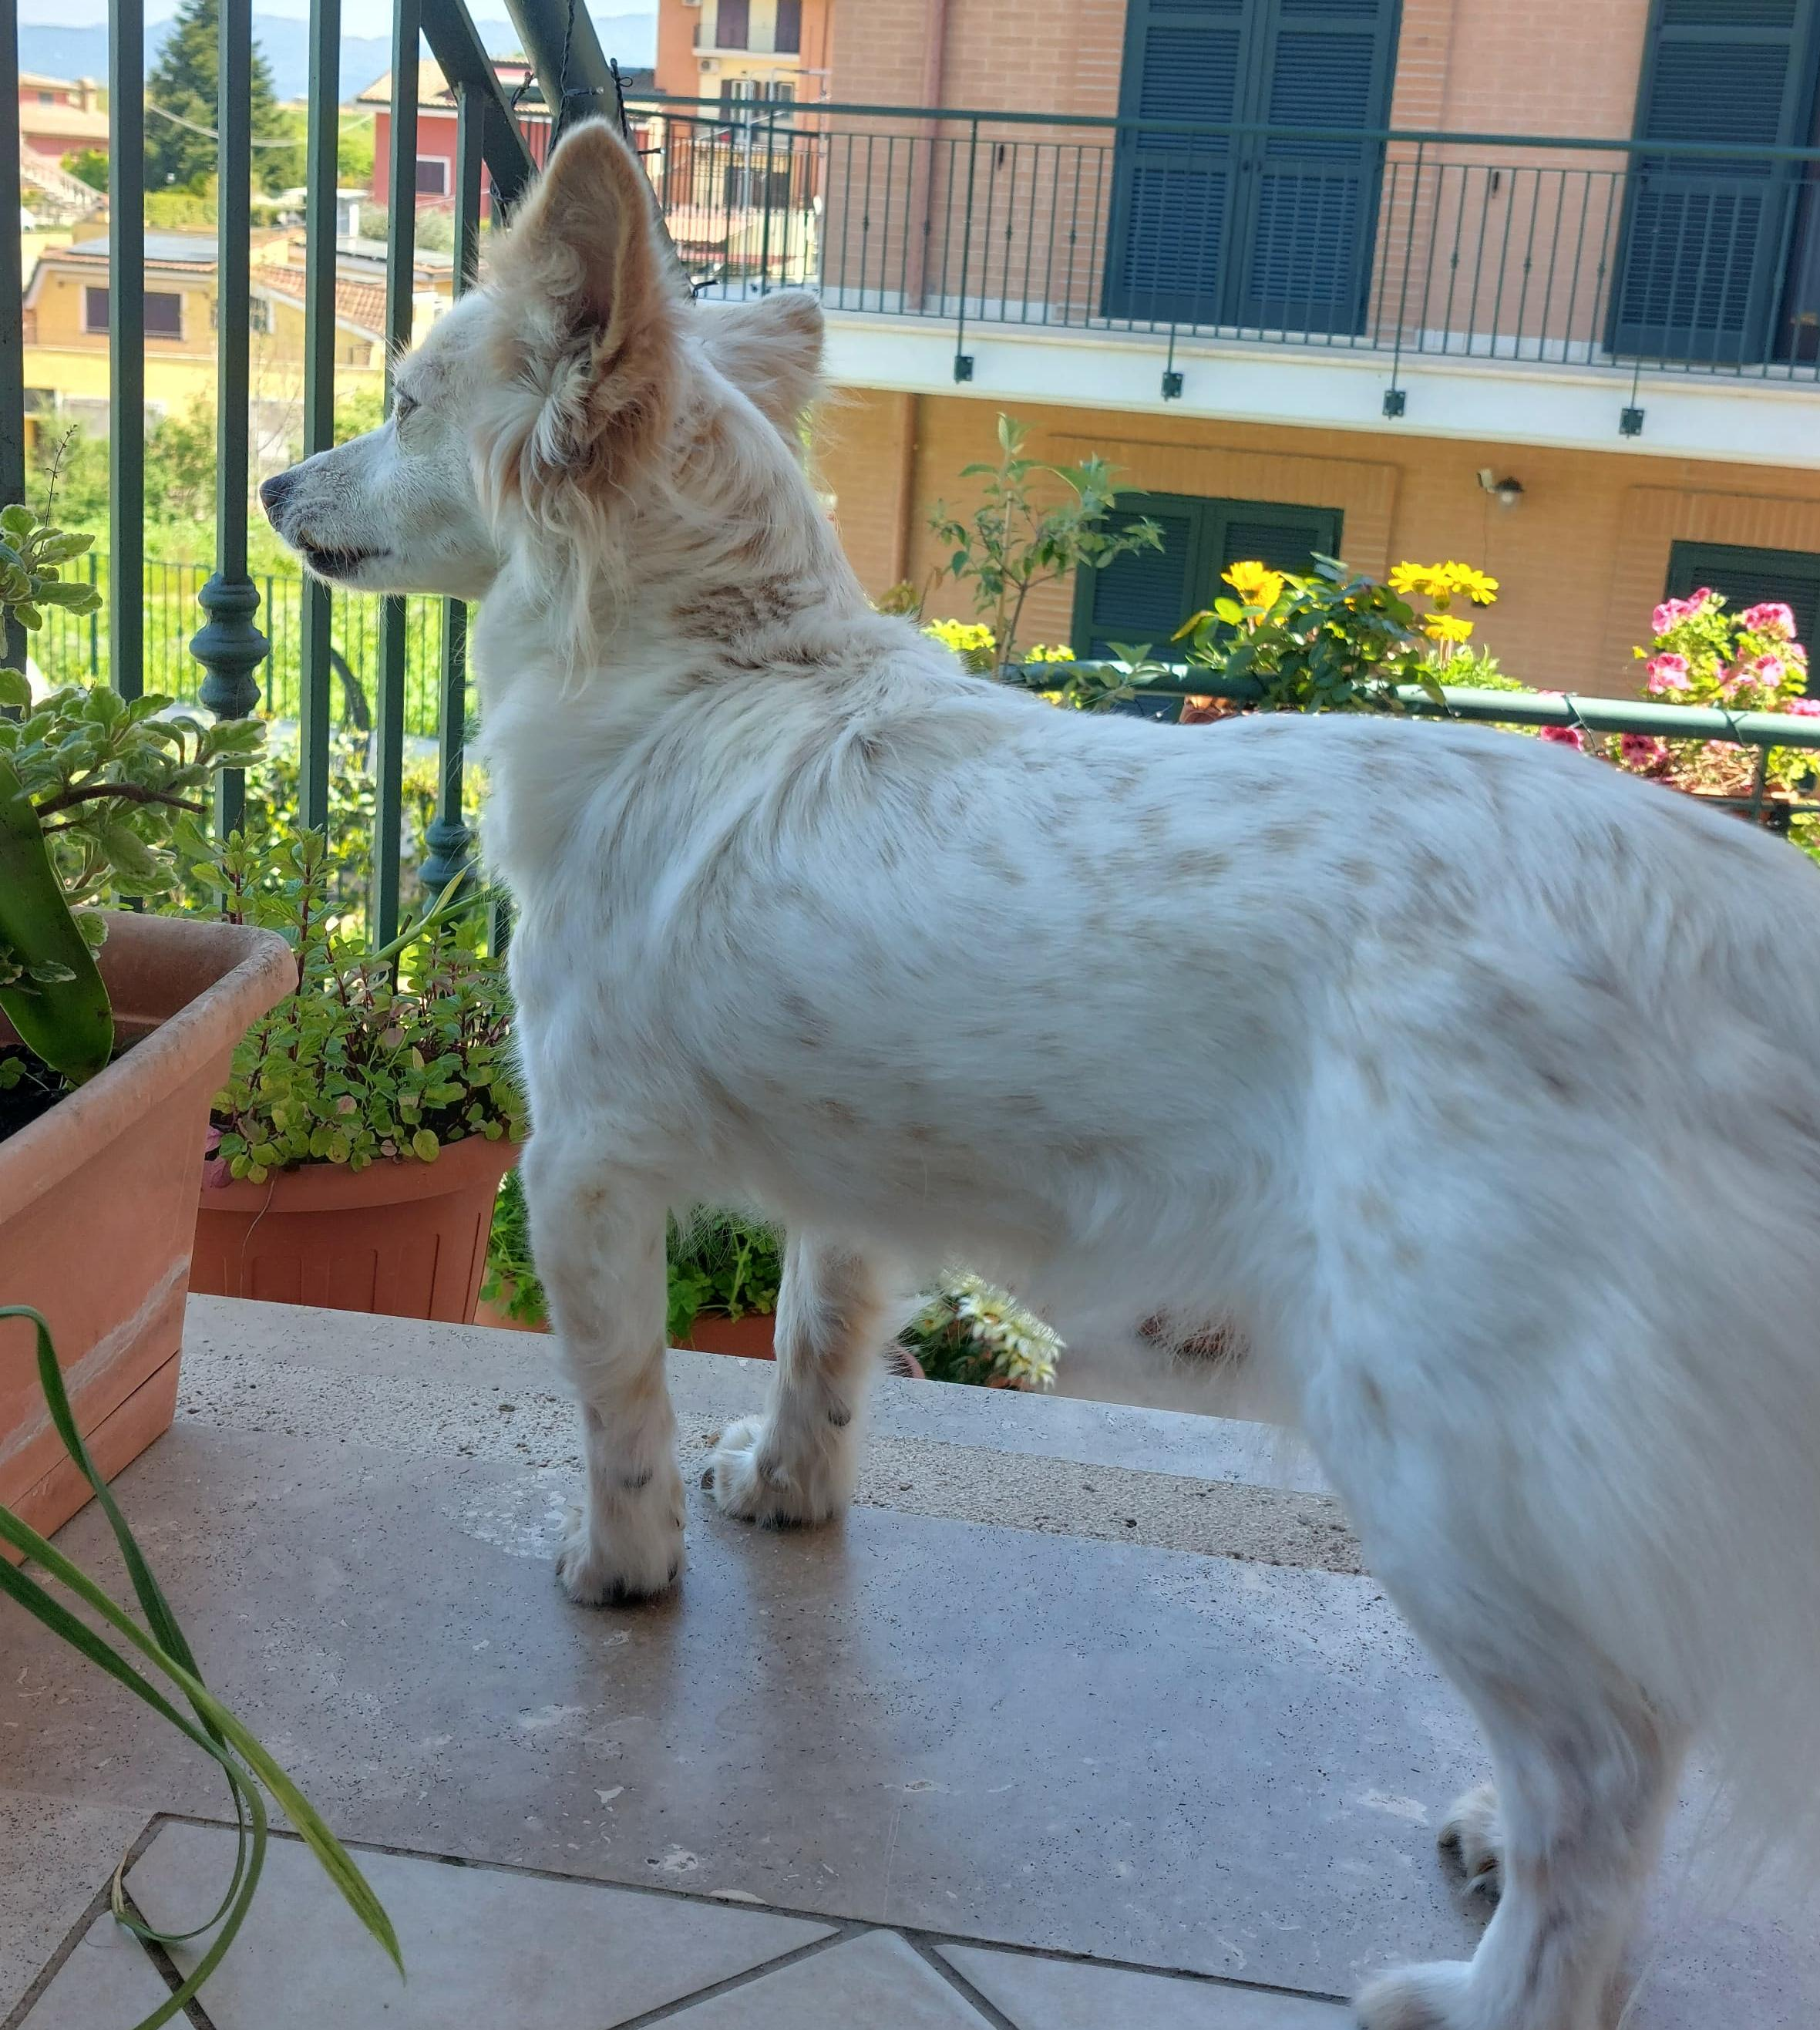
\includegraphics[width=\linewidth]{Figures/example.jpeg}
	\end{subfigure}
	\hspace{2cm}
	\begin{subfigure}{0.4\linewidth}
		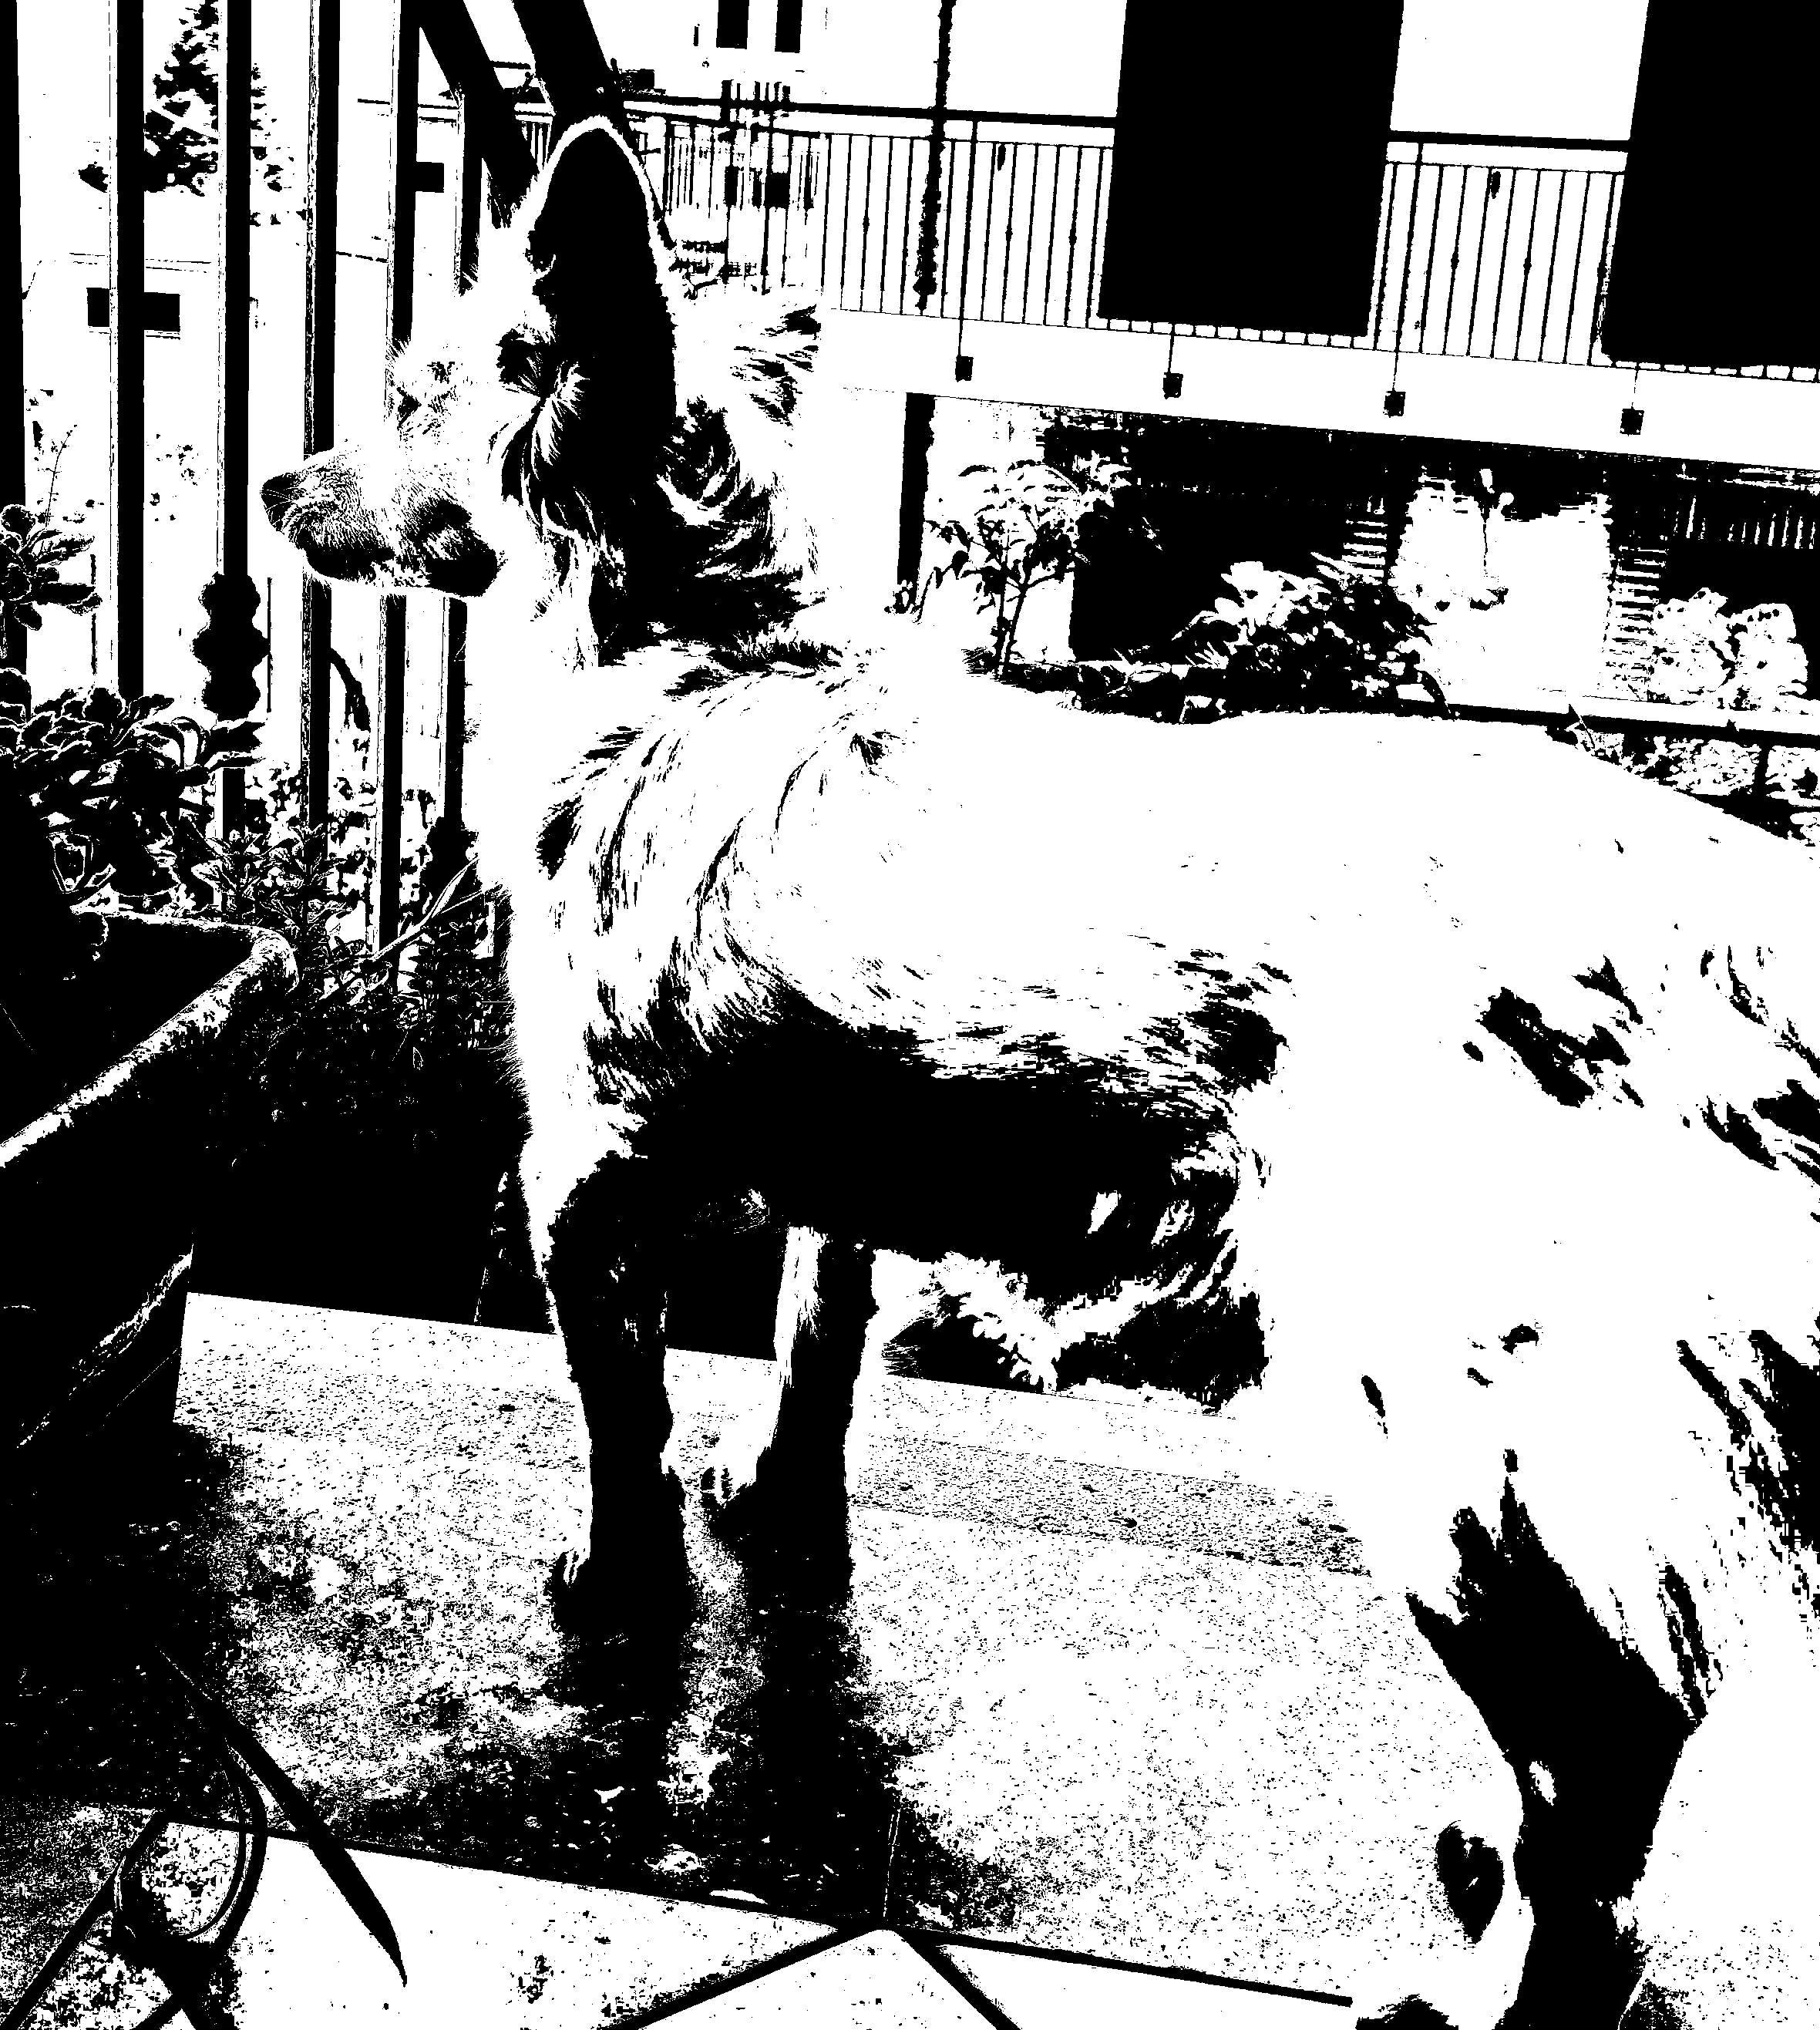
\includegraphics[width=\linewidth]{Figures/example_bw.jpeg}
	\end{subfigure}
	\caption[Example of conversion from RGB to BW]{Example of a conversion from a coloured image to an image with only black and white (bw) pixels. The image is transformed to greyscale by reducing the saturation, finally half of the lightest pixels are rendered white and the remaining are rendered black.}
	\label{fig:example_bw}
\end{figure}

\noindent The research concluded with promising results, showing that the automatic analysis of handwriting samples allows very precise author attributions. However, it turned out that applying the same analysis to pictorial works such as panels and drawings does not produce satisfactory results. It was conjectured that this is due to the intrinsic nature of pictorial works, where the presence of colour plays an important role, and posterisation, instead of helping attribution, generates noise and new information that make the representation of data unreliable.

\begin{note} in questo paragrafo vorrei solo introdurre il concetto di \gls{dada}, potrei parlare di più della tesi triennale in literature review. \end{note}

\paragraph{\gls{cada}}
%Seguendo la stessa linea di ricerca della tesi di \begin{toDo} inserire riferimento \end{toDo}, abbiamo proposto un riadattamento della metodologia al fine di indagare su quale possa essere la strategia più efficace per l'analisi automatica di immagini caratterizzate da un vasto alfabeto di colori. L'obiettivo è costruire una \gls{cada} che possa analizzare i colori nel loro spazio naturale, ovvero in uno spazio continuo. Ciò ci consentirà di superare il vincolo del discreto di \gls{dada} e di ottenere risultati più accurati e dettagliati.
Following the same line of research \cite[my bachelor thesis]{thesis}, we have proposed a re-adaptation of the methodology in order to investigate what might be the most effective strategy for the automatic analysis of images characterised by a large alphabet of colours. The aim is to construct a \gls{cada} that can analyse colours in their natural space, i.e. in a continuous space. This will allow us to overcome the discrete constraint of \gls{dada} and obtain more accurate and detailed results.

\begin{note} lavoro in scale di grigi, ma è comunque uno spazio continuo \end{note}

\noindent Image analysis in \gls{dada} is a process in five stages: acquisition, pre-processing, synthesis, comparison and attribution. In this paper we are going to focus on the first four phases, detailing the process up to image comparison, while attribution will be briefly discussed as the concluding phase.

\noindent The acquisition phase digitises two-dimensional works of art by scanning or photography. Scanning, in particular, allows a high resolution and accurate representation of the original document, while photography allows greater flexibility when the size of the work or physical conditions make scanning complex. The result of this phase is a digital image that accurately represents the work to be analysed.

\noindent The pre-processing phase prepares the image for analysis by removing irrelevant elements through pixel-wise and work-size transformations. Pixel-wise techniques, such as greyscale conversion, act on each individual pixel. Work-size transformations, on the other hand, act on the image as a whole, e.g. with compression techniques or normalisation of colour scales.

\noindent The synthesis phase deconstructs the image into a list of tiles of size $N\times N$, generating a sequence of discrete elements representing portions of the image. This process, aligned with the idea of n-gram language models, allows stylistic features to be analysed in a $\mathbb{R}^{N^2}$ space, preparing the data format for later comparison.

\noindent In the comparison phase, we are going to address the real computational and theoretical challenge. Clustering techniques will be used to dynamically discretise the space of tiles and organise them according to similarity criteria. This allows us both to efficiently process the large number of tiles in a very high dimension and also to compare the target work with known works in the database.

\noindent Finally, in the attribution phase, the similarities between the target work and known works are examined. The aim is to identify the author of the target work by studying the closest works in terms of stylistic and compositional characteristics. This phase focuses on identifying the works that show the greatest stylistic affinity with the target work, suggesting possible attributions.

%(aggiunto direttamente in inglese)
\noindent This research not only aims to tackle technical and computational challenges, but also to explore new perspectives in the analysis of artworks, thus opening up new horizons in the field of art criticism and art attribution.

% acquisition and dataset details
\section{Data Set}
\subsection{Description}
In this study, the data set consists of a set of graphic works for which attribution is established and unambiguous and for which a uniform resolution expressed in \gls{dpi} is known. It was decided to use calligraphic works, as evidenced in \cite{thesis}. The use of calligraphic works represents a promising first way for artistic attribution.

\noindent The dataset used in the reference article consisted of authentic and unaltered handwriting samples. In this study, the dataset consists of university notes, which do not have a sufficiently high standard and therefore present some significant challenges:

\begin{itemize}
\item \textbf{The squares}: Note sheets often contain small squares that could be mistaken for the author's handwriting. This visual interference can complicate the attribution process.
\item \textbf{Use a variety of writing tools}: University notes can be written using a variety of writing tools, such as highlighters, markers, pencils or white-out. These different writing tools produce different lines and colours, which can affect the attribution of authorship.
\item \textbf{Different graphical contexts}: Notes can contain a variety of elements such as mathematical formulae, graphs and erasures. These features represent heterogeneous graphical contexts that add complexity to the analysis.
\item \textbf{Scanning contamination}: The quality of the page scan can introduce blemishes into the record. These blemishes, such as stains or blurring, can affect the clarity and legibility of the works.
\end{itemize}

\noindent In addition, the use of a pen with a thickness of $0.4\operatorname{\mathrm{mm}}$ on the sheet was considered a reasonable first choice since in \cite{thesis} the stroke had the same thickness. This particular aspect is also important in ensuring a certain uniformity and consistency in the visual attributes of the works under examination, thus facilitating a more accurate attribution of authorship.

\noindent The dataset is organised into $4$ authors, and the included images are as follows:

\begin{itemize}
\item The images are saved in the \gls{png} format.
\item Each image is composed of three colour channels \gls{rgb}, each with a depth of 8 bits.
\item The original sheets were scanned at a resolution of 400 \gls{dpi}.
\item The thickness of the pen used to write on the original sheets is $0.4\operatorname{\mathrm{mm}}$.
\end{itemize}

\noindent The images were then cut to remove large impurities or large white spaces. Finally leaving a total of $420$ images.

\begin{table}[h]
    \centering
    \begin{tabular}{|>{\columncolor{pink}}c|c|c|c|}
        \hline
        \rowcolor{lavender}
        \cellcolor{mint} AuthorID & Num of items & Size & Mean side length \\
		\hline
        $1$ & $270$ & $554\operatorname{\mathrm{MB}}$ & $\num{1.43}\operatorname{\mathrm{Kpx}}$ \\
        \hline
        $2$ & $43$ & $133\operatorname{\mathrm{MB}}$ & $\num{1.8}\operatorname{\mathrm{Kpx}}$ \\
        \hline
        $3$ & $56$ & $227\operatorname{\mathrm{MB}}$ & $\num{2.0}\operatorname{\mathrm{Kpx}}$ \\
        \hline
        $4$ & $51$ & $247\operatorname{\mathrm{MB}}$ & $\num{2.2}\operatorname{\mathrm{Kpx}}$ \\
        \hline
        \hline
        \cellcolor{mint} Total & $420$ & $1.2\operatorname{\mathrm{GB}}$ & $\num{1.7}\operatorname{\mathrm{Kpx}}$ \\
        \hline
    \end{tabular}
    \caption[Summary of dataset]{Each item is a cleaned area of the original images. The size represent the total number of pixels. The last column is the geometric mean of the side length, it's compute as follow: $\sqrt{\frac{\text{Num of pixels}}{\text{Num of items}}}$}
\end{table}

In the dataset creation, full clipboard images were collected and then cut to exclude non-pen strokes, highlights, and erasures. In addition, some cuts are particularly small and in a few cases are slightly overlapping.

\begin{figure}[h]
    \centering
    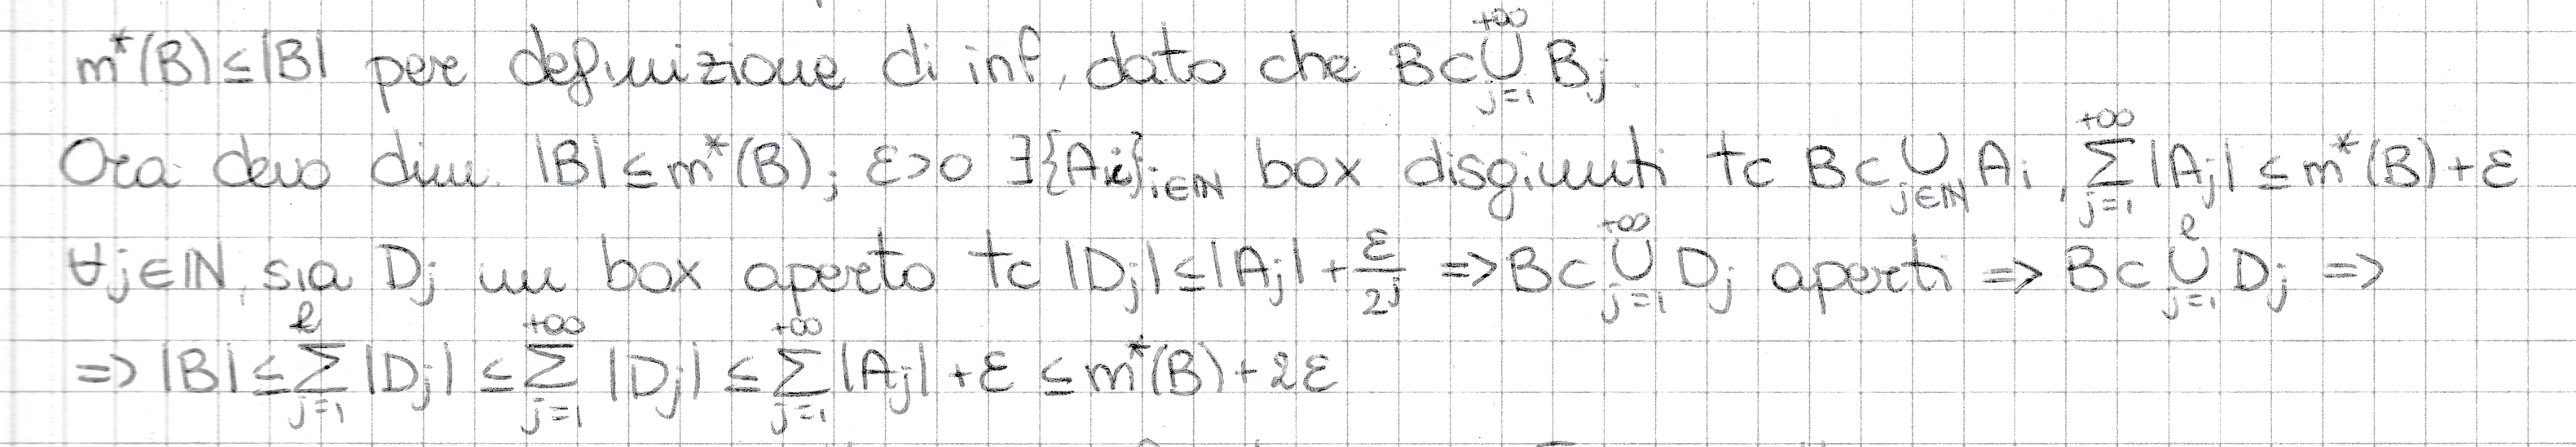
\includegraphics[width=\linewidth]{Figures/Author1_0001_02.png}
\end{figure}


% pre-processing and digitisation theory
\section{Pre processing}
\begin{figure}[ht]
    \centering
    \begin{subfigure}{0.4\linewidth}
        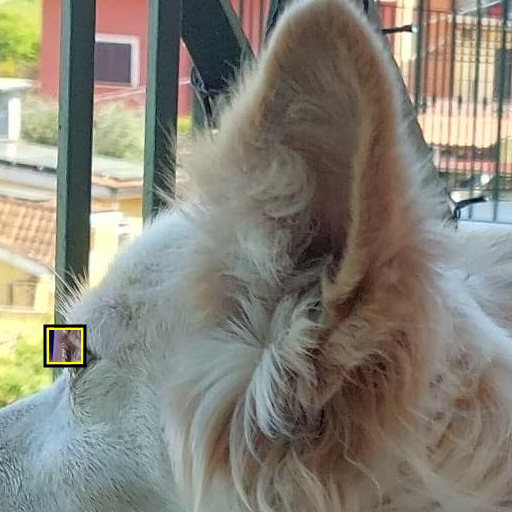
\includegraphics[width=\linewidth]{Figures/example_square.png}
    \end{subfigure}
    \hspace{2cm}
    \begin{subfigure}{0.4\linewidth}
        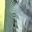
\includegraphics[width=\linewidth]{Figures/example_detail.png}
    \end{subfigure}
    \caption[Pixel grid detail]{Image detail.}
    \label{fig:example_detail}
\end{figure}

%La digitalizzazione delle immagini è un passo fondamentale per preparare le opere d'arte alle analisi che verranno effettuate. Per comprendere appieno il funzionamento di queste trasformazioni, è importante acquisire una conoscenza approfondita del processo attraverso cui un'opera pittorica viene catturata da una macchina fotografica e successivamente digitalizzata in un dispositivo elettronico.
Digitising images is a fundamental step in preparing the data set for analysis. To fully understand how these transformations work, it is important to understand the process by which a work of art is captured by a camera and then digitised in an electronic device.

\paragraph{Definition of image: from the real world to the virtual world}
%Gli artisti dell'antichità utilizzavano varie tecniche, come la camera oscura e i principi della geometria proiettiva, per rappresentare i paesaggi in modo realistico. Durante il Rinascimento, hanno ulteriormente perfezionato questi metodi con strumenti come la camera lucida, mostrando una comprensione matematica avanzata in opere d'arte come la Scuola di Atene di Raffaello.\begin{toDo} citare fonte \end{toDo}.
Artists of antiquity used various techniques, such as the camera obscura and the principles of projective geometry, to represent landscapes realistically. During the Renaissance, they further refined these methods with tools such as the camera lucida, showing advanced mathematical understanding in works of art such as Raphael's School of Athens.\footnote{for more about camera obscura, see\newline\url{https://en.wikipedia.org/wiki/Camera_obscura}}

%\noindent L'invenzione della fotografia nel $1826$, in concomitanza con il movimento artistico del Realismo, segnò un momento fondamentale nella storia dell'arte visiva. La fotografia, con la sua capacità di rappresentare la realtà in modo oggettivo, divenne uno strumento sempre più utilizzato dagli artisti. L'avanzamento delle conoscenze in ottica e chimica portò alla creazione della fotografia analogica \begin{toDo} citare fonte e inserire immagine \end{toDo}.
\noindent The invention of photography in $1826$, in conjunction with the art movement of Realism, marked a fundamental moment in the history of visual art. Photography, with its ability to represent reality objectively, became a tool increasingly used by artists. The advancement of knowledge in optics and chemistry led to the creation of analogue photography.\footnote{for more about history of photography, see\newline\url{https://en.wikipedia.org/wiki/History_of_photography}}
\begin{figure}[ht]
    \centering
    \begin{subfigure}[t]{0.4\linewidth}
        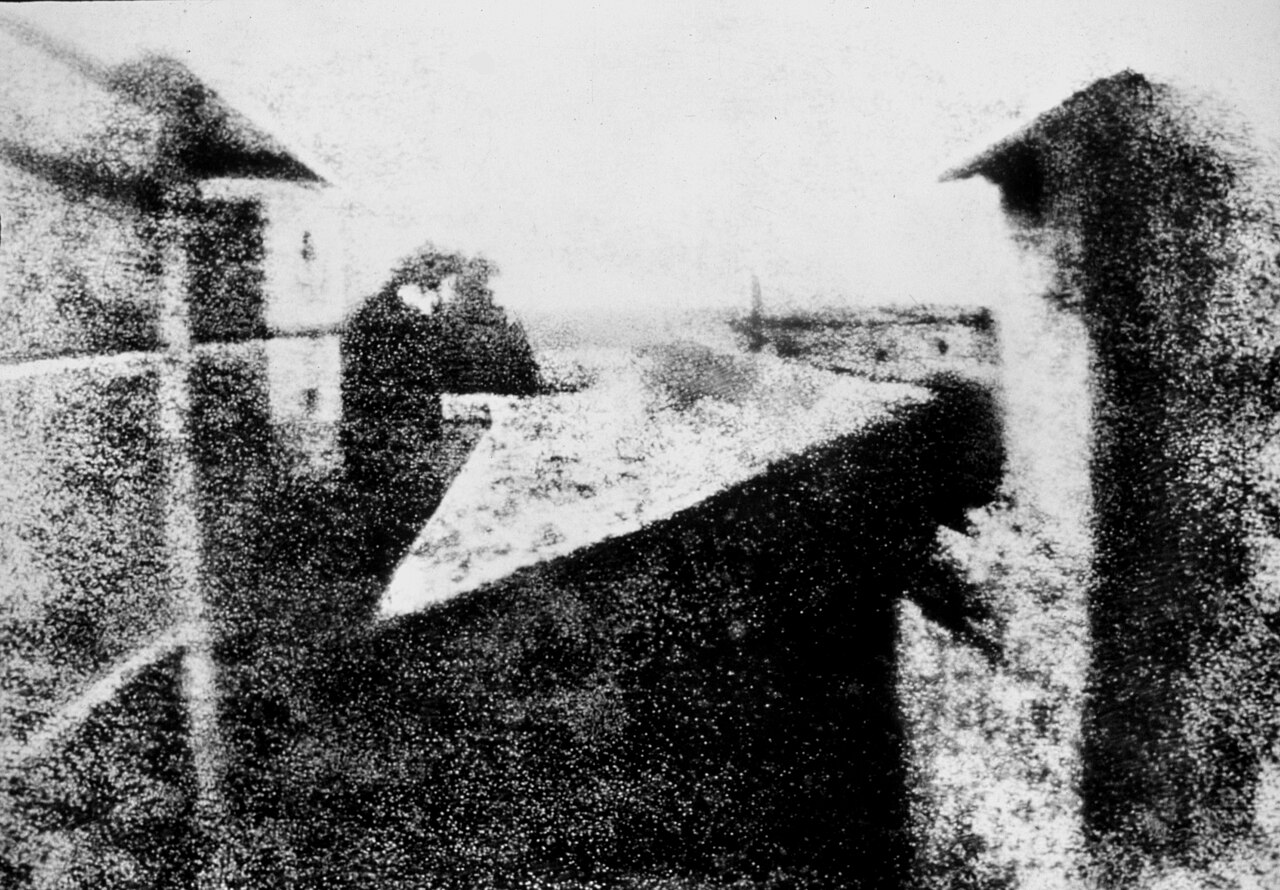
\includegraphics[width=\linewidth]{Figures/FotoStoria.jpg}
        \caption{'View from the Window at Le Gras', Joseph Nicéphore Niépce, c.1826, Heliography, Harry Ransom Center, University of Texas at Austin, USA\cite{FirstPhoto}.}
    \end{subfigure}
    \hspace{2cm}
    \begin{subfigure}[t]{0.4\linewidth}
        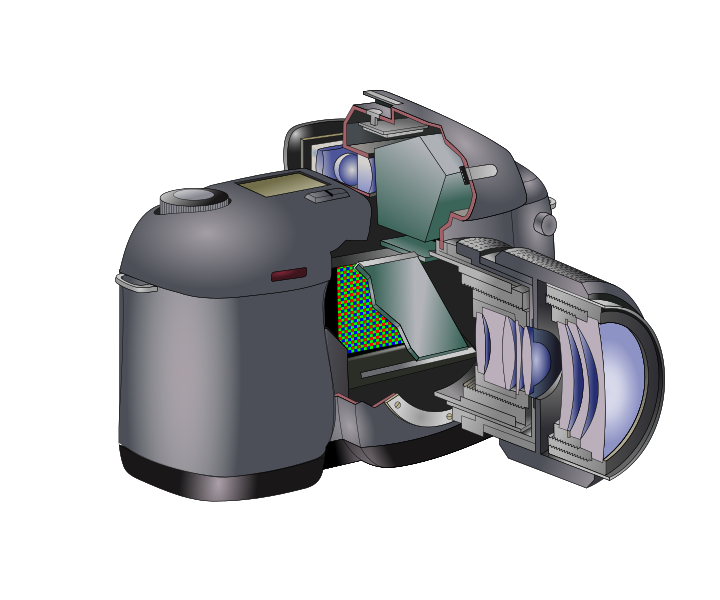
\includegraphics[width=\linewidth]{Figures/digitalcamera.png}
        \caption{Illustration of digital camera\cite{Reflex}.}
    \end{subfigure}
\end{figure}

%\noindent Nel corso degli anni ottanta, con l'avvento della tecnologia informatica, la fotografia digitale divenne una realtà. Il funzionamento di base rimase simile alle tecniche precedenti, ma con l'aggiunta di un nuovo processo di digitalizzazione. Invece di essere impressa su una superficie fotosensibile, l'immagine viene catturata da una griglia di sensori ottici e digitalizzata come una matrice di colori, con ogni componente chiamata "pixel" \begin{toDo} inserire fonte e immagine \end{toDo}.
\noindent During the 1980s, with the advent of computer technology, digital photography became a reality. The basic operation remained similar to previous techniques: instead of being printed on a photosensitive surface, the image was captured by a grid of optical sensors and digitised as a matrix of colours, with each component called a pixel.

%\noindent Il concetto di riproduzione dei colori non è nuovo, e già nel $1855$ James Clerk Maxwell lavorò su questo tema, introducendo il modello di colore \gls{rgb}, ancora oggi ampiamente utilizzato. Questo modello codifica ogni colore con tre numeri reali in un intervallo tra $0$ e $1$. Tuttavia, per scopi informatici, si è convenuto di rappresentare i $3$ valori di un colore con numeri interi compresi tra $0$ e $255$ \begin{toDo} inserire fonte per lavoro di Maxwell \end{toDo}. In questo modo, un'immagine digitale diventa una matrice di triple, rappresentando i valori dei pixel nei tre canali di colore \gls{rgb}.
\noindent The concept of colour reproduction is not new and as early as $1855$ James Clerk Maxwell worked on this subject, introducing the colour model \gls{rgb}, which is still widely used today (see \cite{MaxWell_Colours}). This model encodes each colour with three real numbers in an interval between $0$ and $1$. However, for computing purposes, it was agreed to represent the $3$ values of a colour with integers between $0$ and $255$. In this way, a digital image becomes a matrix of triples, representing the pixel values the three colour channels \gls{rgb}.

\subsection{Grayscale reduction}
The quantisation of colours is expressed in $3$ channels \gls{rgb}, each with an integer value between $0$ and $255$. The choice of these $3$ colours is not arbitrary; it derives from a physiological feature of human vision. Our perception of colour is determined by photoreceptor cells in the eye called cones, of which there are three types: S-cones, M-cones and L-cones. These cones are sensitive to wavelengths that approximately correspond to blue, green and red light respectively.

\noindent This model of colour representation is therefore deeply rooted in the way our visual system works, rather than in the physical reality of light. For example, when we see yellow, it is the result of the simultaneous activation of both M and L cones, which our brain interprets as a pure yellow colour. This perception is not a direct consequence of the physical properties of light, but rather a result of our brain's processing. Similarly, the colour magenta does not have a single wavelength in the visible spectrum, but is perceived when our brain combines stimuli from both red and blue wavelengths. These examples illustrate that colour perception is a subjective phenomenon in which the brain combines signals in a way that does not always reflect a direct physical counterpart.

\noindent This subjective nature of colour perception means that our representation of colour space is influenced more by neurological processes than by physical reality. While physically we might think of colour as occupying a continuous, structured space (e.g. a cone or cylinder in RGB representation), the actual experience of colour varies between individuals. For example, people with colour blindness may perceive certain colours differently due to differences in their cones. In addition, cultural differences can also affect perception: the Himba people of Namibia, for example, can distinguish between shades of green that many others cannot, while they may have difficulty distinguishing green from blue\footnote{For more about Himba people, see \url{https://en.wikipedia.org/wiki/Himba_people}}.

\noindent Given this subjective interpretation, the classification of colours often goes beyond a purely scientific approach. In contexts such as art, where perception and expression are key, it is often more useful to refer to colour spaces such as \gls{hsl}, which represent hue, saturation and lightness, rather than the more physically oriented \gls{rgb}. These spaces provide a more intuitive way of describing how colours relate to each other in terms of what we actually perceive.

\noindent Greyscale reduction builds on this understanding of colour perception. It involves reducing the image to the brightness component only, effectively removing hue and saturation. There are several techniques to achieve this. One common method is to take a weighted average of the three RGB channels, with the weights chosen to reflect the varying sensitivity of the human eye to different colours. Another approach is to average between the maximum and minimum intensity channels. Whatever the method, the aim is to create a representation of the image that retains luminance information while discarding colour, thus simplifying the visual data while retaining the essence of light intensity.

\begin{figure}[h]
    \centering
    \begin{subfigure}[t]{0.4\linewidth}
        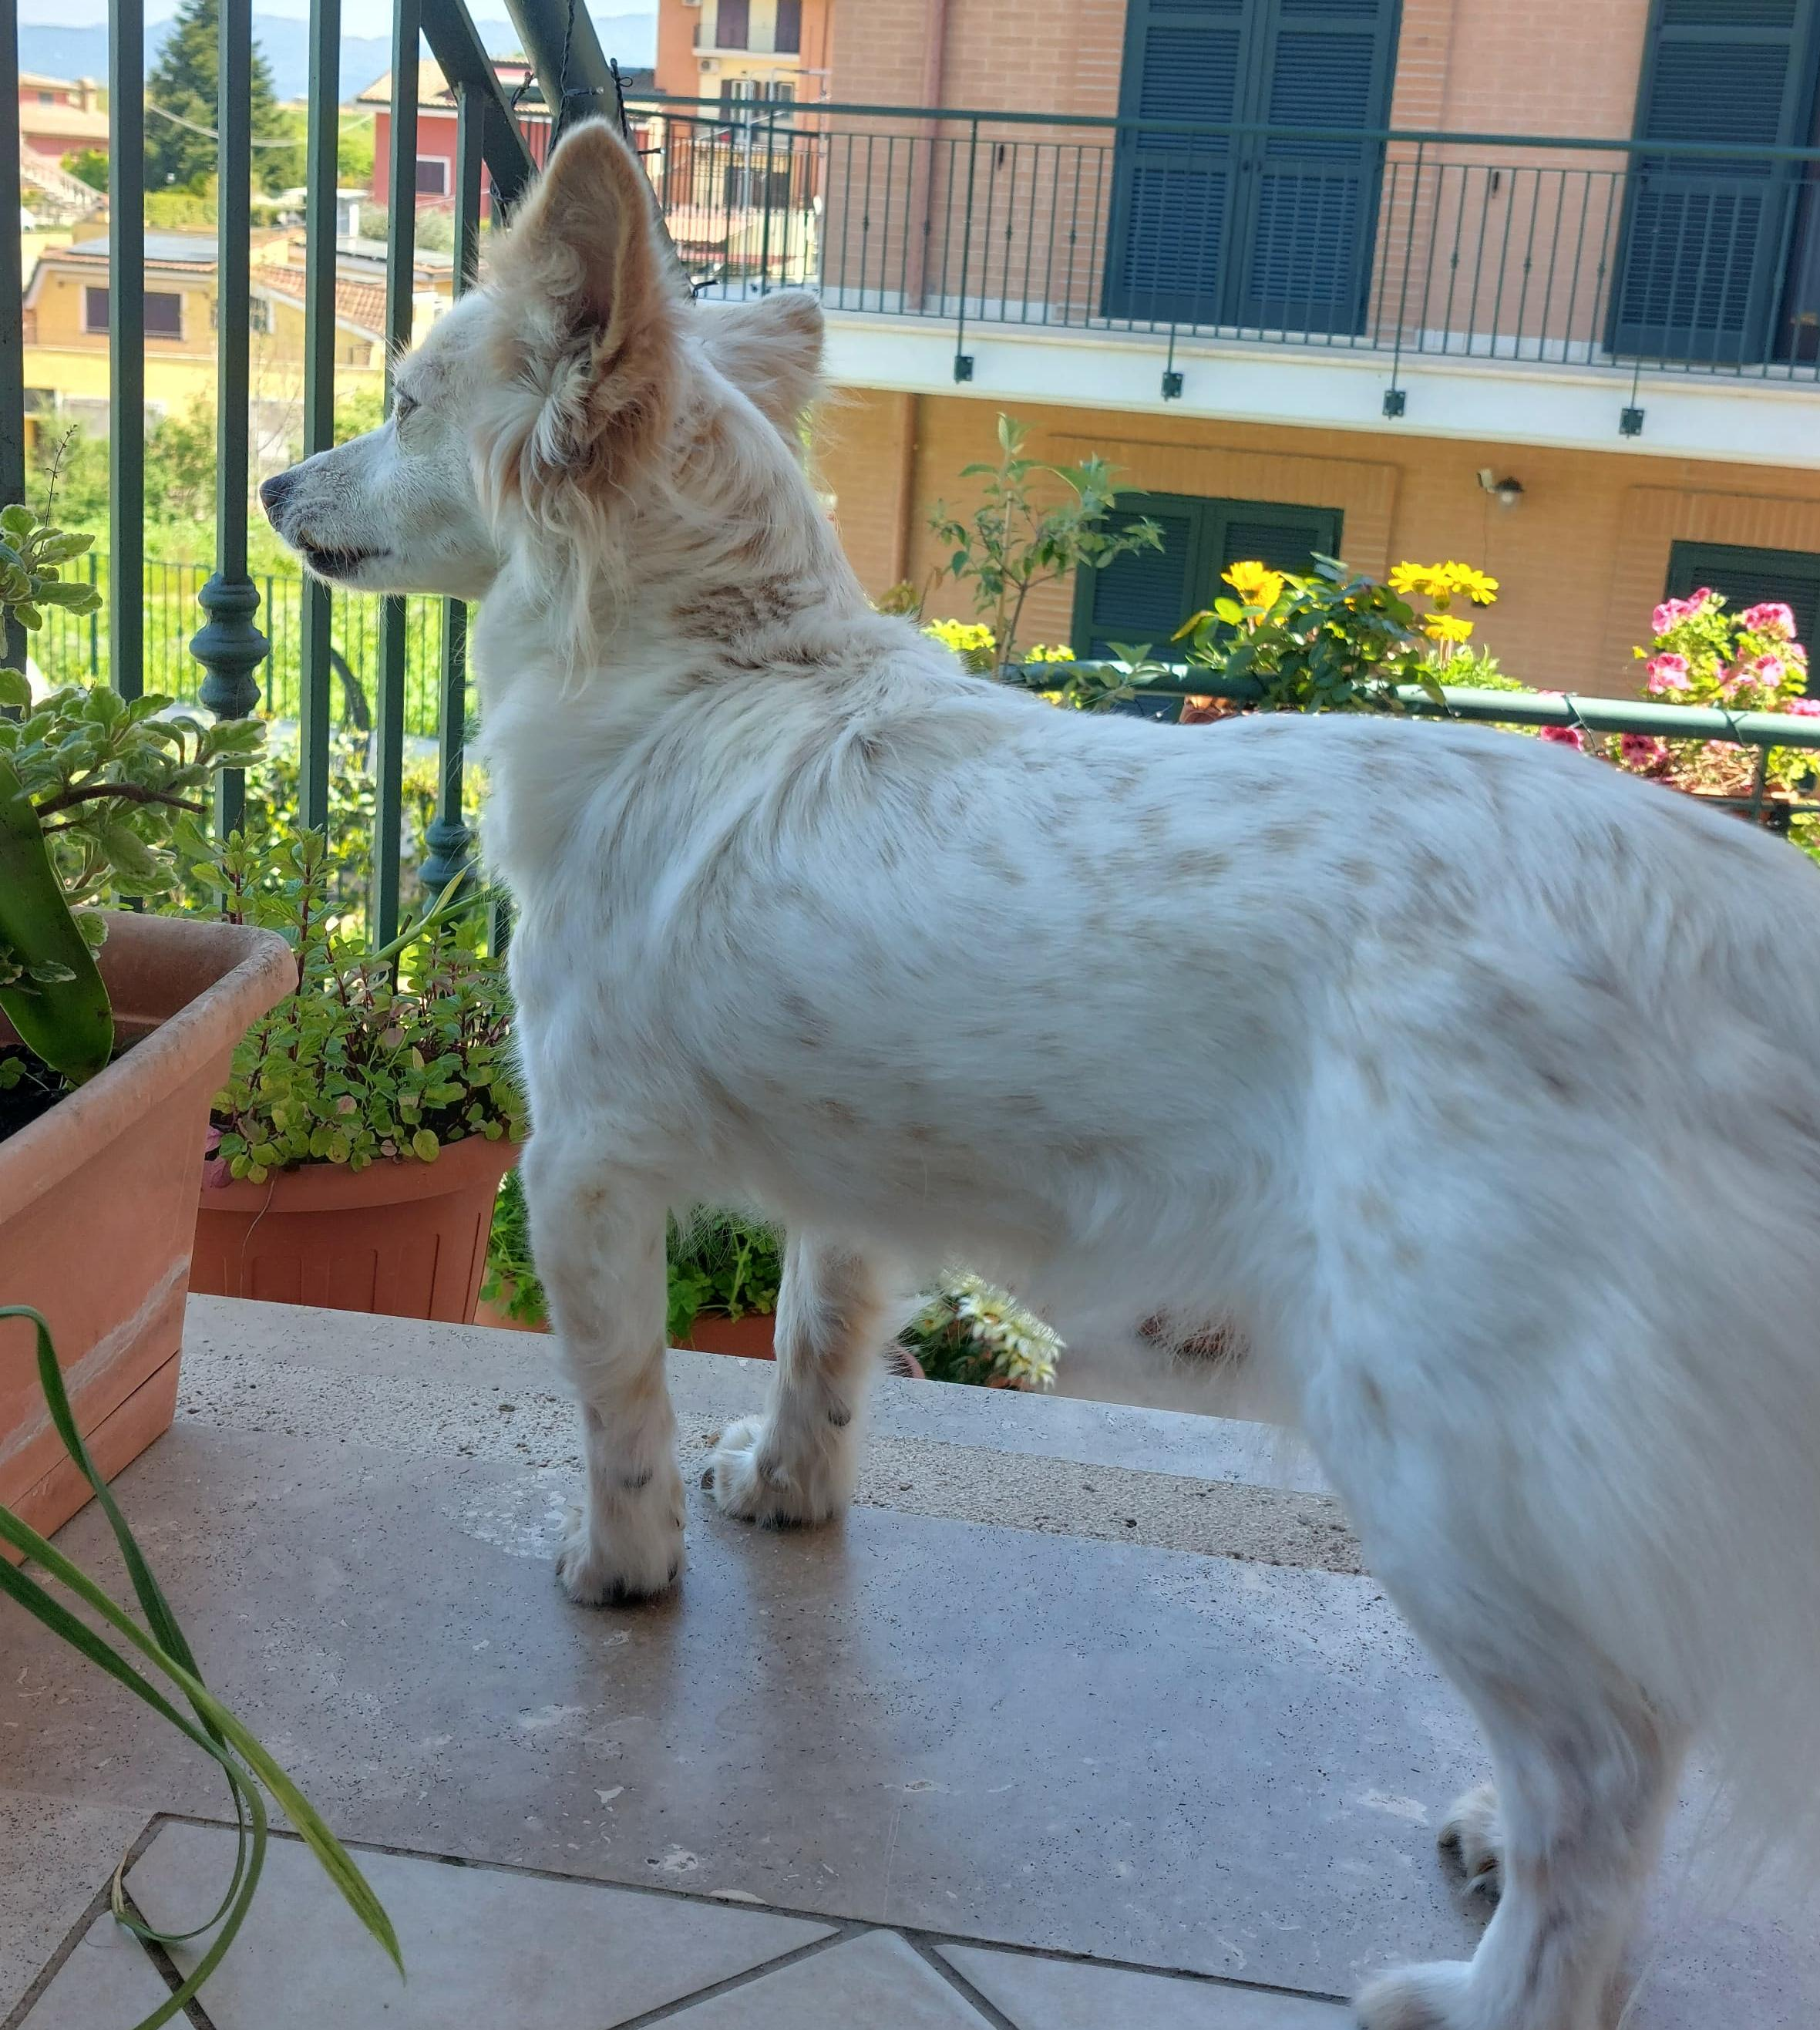
\includegraphics[width=\linewidth]{Figures/example.jpeg}
    \end{subfigure}
    \hspace{2cm}
    \begin{subfigure}[t]{0.4\linewidth}
        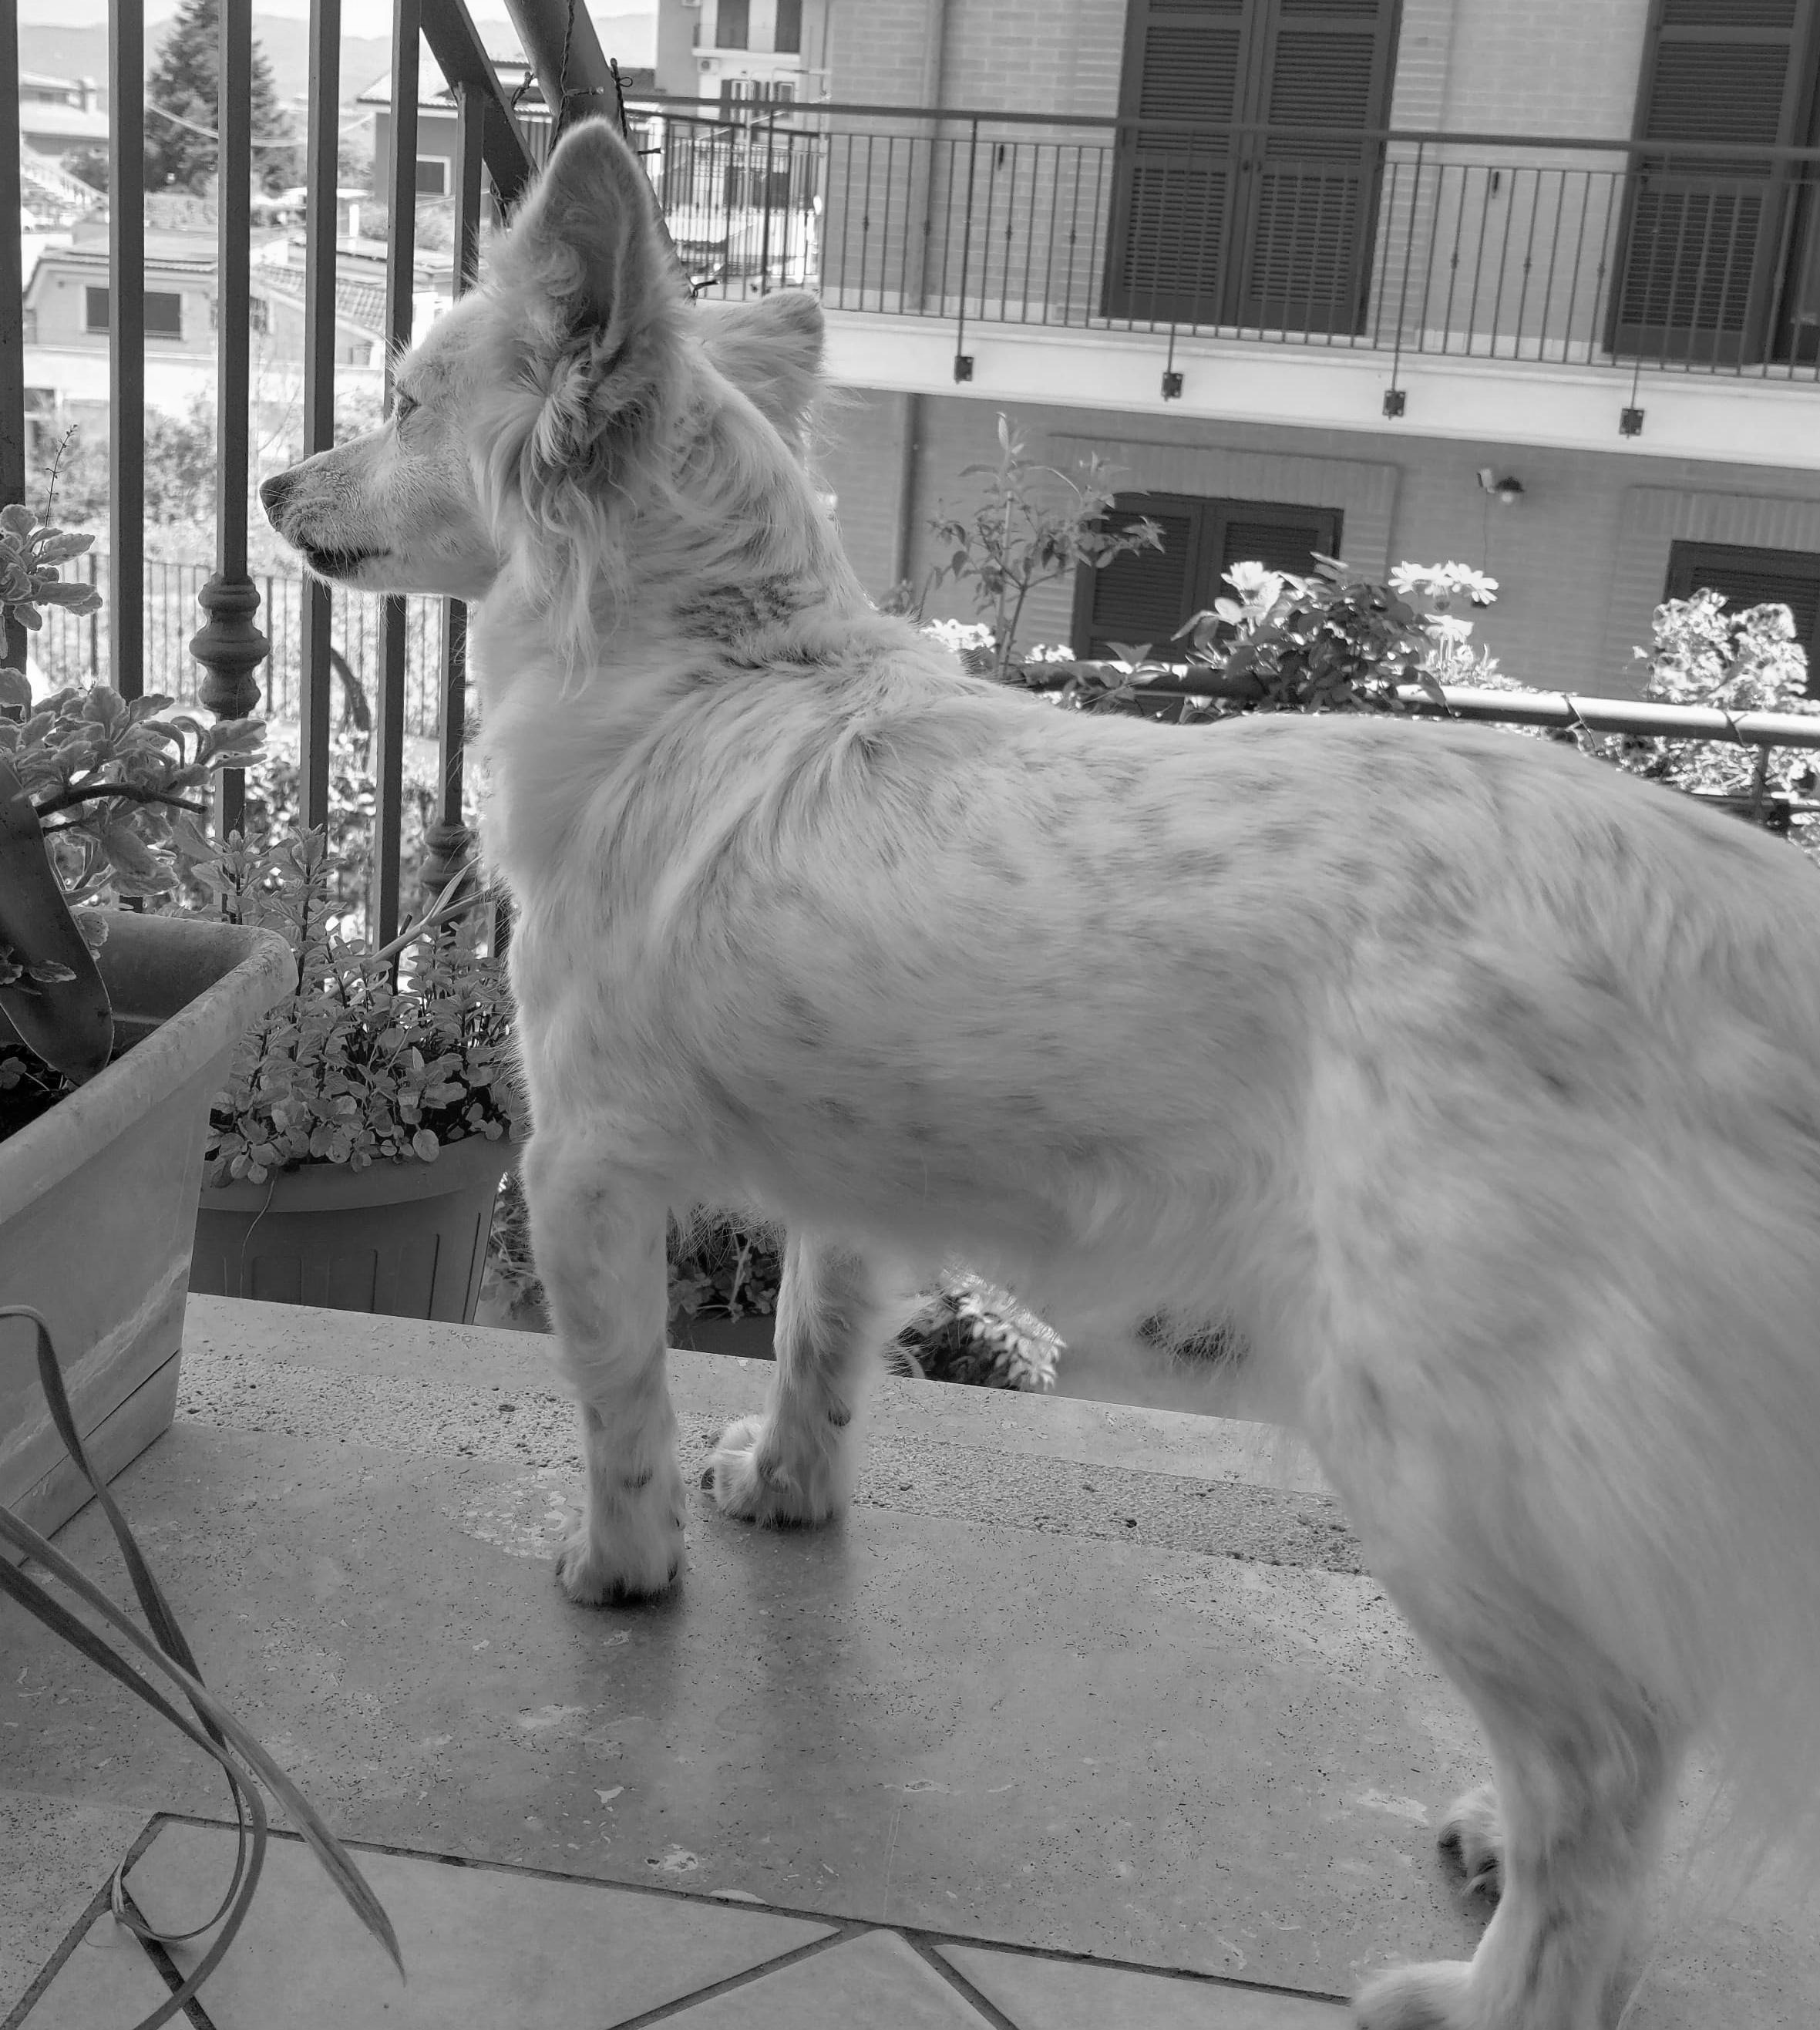
\includegraphics[width=\linewidth]{Figures/example_gray.jpeg}
    \end{subfigure}
\end{figure}
\subsection{Removing squares}
    One of the main challenges in processing and collecting the dataset concerns the cleanliness of the images, which can have significant impurities, such as the presence of squares on the sheets. It is essential to remove or mitigate these elements so that they blend in with the background and do not interfere with the analysis. Initially, the use of static techniques such as thresholding or the application of specific kernels to recognise the squares was considered. However, such techniques risked compromising the author's writing by erasing details. For this reason, it was decided to use compression techniques to detect patterns, since squares constitute a highly visible pattern that is more easily distinguishable by the machine than human handwriting.

    \paragraph{\gls{svd}}
    A first test involved examining the predominant patterns by means of a decomposition \gls{svd}. The image can be viewed as a matrix $H \times W$ of real values and can be decomposed into the product:
    \[
    	U\Sigma V^H = M
    \]
    where $M$ represents the image, $U$ and $V$ are unitary matrices ($UU^H = I$, same for $V$), $V^H$ is the Hermitian of $V$, and $\Sigma$ is a matrix $H \times W$ with only real values along the diagonal, called singular values.\
    It is possible to obtain a less detailed version of $M$ by cancelling some singular values of $\Sigma$, thus ignoring the contribution of certain patterns. It was observed that the predominant pattern (associated with the largest singular value) concerns squares, but its removal does not completely solve the problem, requiring the elimination of further patterns. The result obtained is encouraging, but entails a loss of information from human handwriting, as it too is present among the major patterns identified.

    \paragraph{\gls{fft}}
    An alternative idea is to perform a harmonic analysis of the images using \gls{fft}. The squares are repeated with a specific frequency along the two dimensions of the sheet and thus one can exploit their regular nature compared to human handwriting, which is less repetitive. Thus, one exploits both the difference between the regular patterns of the squares and the irregular strokes of the handwriting, as well as a greater capacity for compression than a simple pixel-by-pixel analysis.

    \noindent To verify this idea, we run a \gls{fft} on test images: a virtual sheet with only squares and the same sheet with drawings on it. In the case of the unmarked sheet, frequencies with larger amplitudes are mainly found aligned along the $x$ and $y$ axes (\cref{fig:synthetic_grid_fft}). By adding a pattern, the main frequencies remain almost the same (\cref{fig:synthetic_sign_fft}). To remove the squares, we remove these significant frequencies and reconstruct the image (\cref{fig:synthetic_clean_fft}).

    \begin{figure}
    	\centering
    	\begin{subfigure}[t]{\linewidth}
    		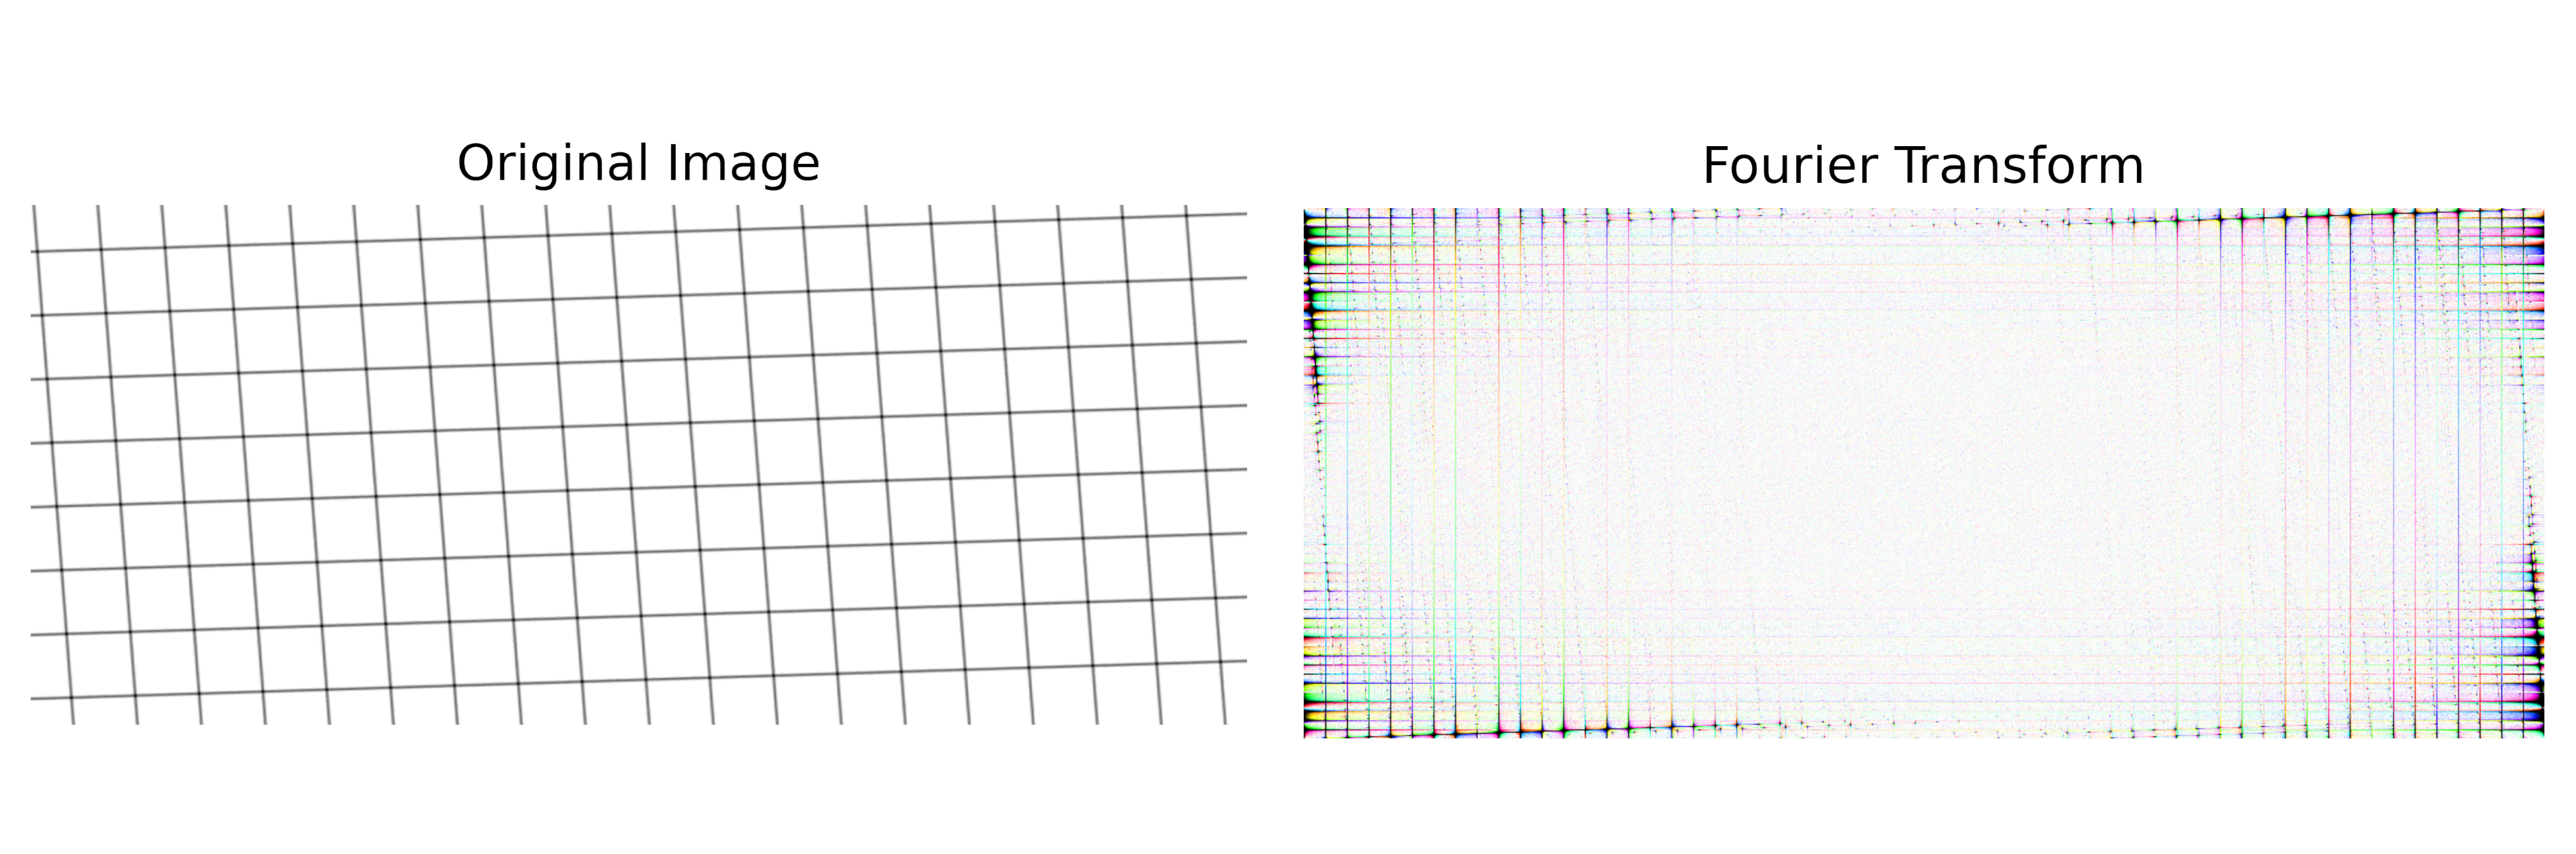
\includegraphics[width=\linewidth]{Figures/grid_fft.png} \caption{A slightly transformed grating, caused by an imperfect scan. The most significant frequencies are highlighted in black.} \label{fig:synthetic_grid_fft}
    	\end{subfigure}
    	\begin{subfigure}[t]{\linewidth}
    		\includegraphics[width=\linewidth]{Figures/test_fft.png} \caption{A deformed grating with a superimposed inscription. The frequencies of the lattice remain visible.} \label{fig:synthetic_sign_fft}
    	\end{subfigure} \begin{subfigure}[t]{\linewidth}
    		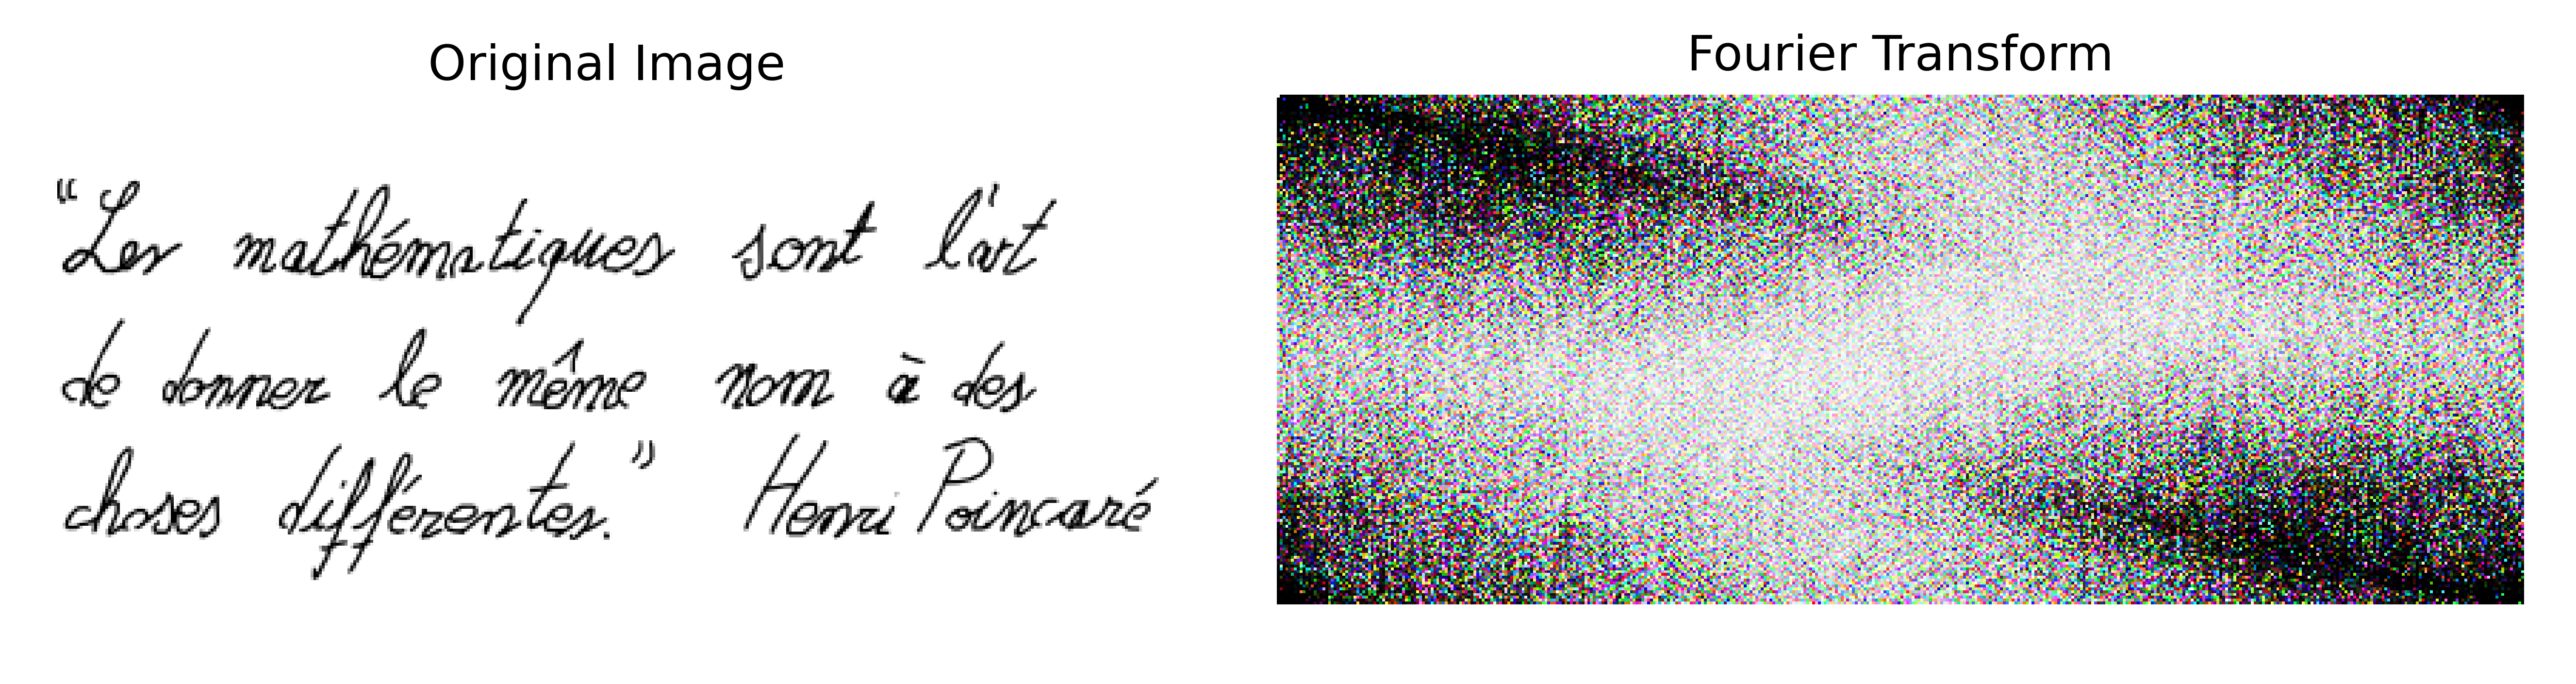
\includegraphics[width=\linewidth]{Figures/clean_fft.png} \caption{Lattice-less writing does not show significant Fourier coefficients, as recurring patterns are missing.} \label{fig:synthetic_clean_fft}
    	\end{subfigure}
    	\caption[Synthetic FFT test]{Fourier coefficient of the two-dimensional image. The squares show Fourier coefficients similar to those of the square waves: $\text{sqwave}(t) = \frac{4}{\pi}\sum_{k=1}^{\infty}\frac{\sin\left(2\pi(2k-1)t\right)}{2k-1}$. The most significant intensities are at regular intervals with decreasing intensities.}
    \end{figure}

    \noindent Empirically, by analysing $10$ randomly selected real images, it was observed that the squares were successfully removed without damaging the lettering, cancelling out the amplitudes corresponding to the first $5\%$ percentile of the most significant frequencies.

    \noindent However, this process introduces an issue of colour distortion. In the original image, the grey levels were distributed intuitively: most of the pixels were white, with only a small portion in darker shades of grey, representing the writing. After reconstructing the image using the FFT, a significant number of pixels took on intermediate shades of grey that weren't present before. This affects the clarity of the image, especially by blending the background and the lettering, making it harder to distinguish between the important features from the unwanted noise.

	\noindent To reduce the effects of this distortion, we adopted a colour normalisation approach to keep the grey values as close as possible to the original image. The main idea was to identify extremely light and extremely dark grey values in the original image and to expand the range of grey values in the reconstructed image to match them.

    \noindent It was observed that, in the original image, pixels with a grey level below $0.2$ certainly belong to the lettering, while those with a grey level above $0.8$ correspond to the white background of the page. Consequently, the pixels of the lettering and white background in the original image are counted. In the cleaned image, the darkest pixels (with a grey value below $0.2$ in the original image) are assigned to black, while the lightest pixels (with a grey value above $0.8$ in the original image) are assigned to white.

    \noindent To correct the distortion, we expanded the grey values of the reconstructed image so that pixels that should be black became darker and those that should be white became lighter. We then clamped these values within natural limits (0 to 1) to avoid out-of-scale colours. This process was called ‘clamp normalisation’. A result of this procedure is shown in \cref{fig:first_reconstruct}.

    \begin{note} Presente nel capitolo Results \end{note}

    \begin{algorithm}[h]
    	\caption[Cleaning procedure using FFT]{Cleaning procedure using FFT.\\
    		\begin{minipage}[t]{\linewidth}
    			\textsc{INPUT}
    			\begin{itemize}[noitemsep, topsep=0pt]
    				\item[$\mathcal{I}$:] Image as matrix $W\times H$ in gray scale
    				\item[$p$:] percentile of significant magnitudes
    				\item[$a$:] thresholds $(\min, \max)$
    			\end{itemize}
    			\textsc{OUTPUT} $\mathcal{I}_{\text{new}}$: Image as matrix $W\times H$ in gray scale
    		\end{minipage}
    	}
    	\begin{algorithmic}[1]
    		\Procedure{CleanFFT}{$\mathcal{I}, p, a$}
    		\State $\hat{\mathcal{I}} \gets \text{normalize}\left(\mathcal{I}\right)$
    		\State $F_{\hat{\mathcal{I}}} \gets \text{fft2d}\left(\hat{\mathcal{I}}\right)$
    		\State $f = (f_1, \dots, f_{W\times H}) \gets \text{argsort}\left(\text{flatten}\left(F_{\hat{\mathcal{I}}}\right), \text{rule=abs}\right)$
    		\State $f_{\text{best}} \gets f\left[\text{last}\; \lfloor{p\cdot\text{length}\rfloor}\;\text{values}\right]$ \Comment{components with high magnitude}
    		\For{$k \in f_{\text{best}}$}
    			\State $F_{\hat{\mathcal{I}}}[k] = 0.0$
    		\EndFor
    		\State $\hat{\mathcal{I}} \gets \text{ifft2d}\left(F_{\hat{\mathcal{I}}}\right)$ \Comment{rebuild normalized image}
    		\State $w_{\text{cnt}} \gets \textbf{count}\;\mathcal{I} \geq a(\max)$ \Comment{normalization using dilation and clamp}
    		\State $b_{\text{cnt}} \gets \textbf{count}\;\mathcal{I} \leq a(\max)$
    		\State $h_{w} \gets \max_{w_{\text{cnt}}^{\mathrm{-th}}}\mathcal{\hat{I}}$
    		\State $h_{w} \gets \min_{b_{\text{cnt}}^{\mathrm{-th}}}\mathcal{\hat{I}}$
    		\State $\mathcal{I}_{\text{new}} \gets \frac{\mathcal{\hat{I}} - h_{b}}{h_{w}-h_{b}}$
    		\Where{$\mathcal{I}_{\text{new}} > 1$, $\mathcal{I}_{\text{new}} = 1$}
    		\Where{$\mathcal{I}_{\text{new}} < 0$, $\mathcal{I}_{\text{new}} = 0$}
    		\State \Return $\mathcal{I}_{\text{new}}$
    		\EndProcedure
    	\end{algorithmic}
    	\label{alg:CleaningFFT}
    \end{algorithm}


% synthesis algorithm
\section{Synthesis}
The tessellation phase extracts tiles $N\times N$ from each image. Starting from a matrix of grey pixels, represented as a matrix in $\left[0,1\right]^{h \times w}$, where $h$ is the height and $w$ the width of the image.

\noindent Al termine di questa procedura, ogni immagine viene rappresentata come un elenco di tessere, motivo per cui questa fase è chiamata "sintesi": infatti, risulta difficile ricostruire l'immagine originale a partire dalle tessere. Questo processo complica notevolmente qualsiasi tentativo di falsificazione dell'opera, poiché ricostruire manualmente un'immagine con una distribuzione di tessere simile a quella originale è estremamente complicato. Inoltre, la dimensione delle tessere nella rappresentazione è ridotta, ma sufficientemente grande da catturare piccoli automatismi della mano dell'autore, dettagli che sono difficilmente riproducibili in modo volontario.

\begin{algorithm}[ht]
\caption{Algorithm for tile extraction}
\begin{algorithmic}[1]
\Function{TilesExtraction}{$\textnormal{M}, \textnormal{h}, \textnormal{w}$}
    \State declare $v$ as matrix $N \times N$ \Comment{$N$ is size of tiles}
    \State $L \gets \texttt{empty list}$ \Comment{will have $(\textnormal{h} - N + 1)\times(\textnormal{w} - N+1)$ elements}
    \For{$row \gets 0$ to $\textnormal{h} - N$, $col \gets 0$ to $\textnormal{w} - N$}
        \For{$i \gets 1$ to $N$, $j \gets 1$ to $N$}
            \State $v[i][j] \gets \textnormal{M}[row + i][col + j]$
        \EndFor
        \State call \texttt{Append}($L$, $v$)
    \EndFor
\EndFunction
\label{alg:SequentialTilesExtraction}
\end{algorithmic}
\end{algorithm}

\begin{figure}[ht]
    \centering
    \begin{subfigure}{0.4\linewidth}
        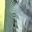
\includegraphics[width=\linewidth]{Figures/example_detail.png}
        \caption{Image detail $32 \times 32$.}
    \end{subfigure}
    \hspace{2cm}
    \begin{subfigure}{0.4\linewidth}
        
\includegraphics[width=\linewidth]{Figures/example_tiles.png}
        \caption{List of tiles $8 \times 8$.}
    \end{subfigure}
    \caption[Illustration of synthesis process]{The synthesis process convert an image in a list of its tiles.}
    \label{fig:puffer_tiles}
\end{figure}


% comparison and theory
\section{Comparison}
\begin{modified}
In order to compare two works, we decided to use the clustering \gls{fcm}, which is less sensitive to potential noise. This is particularly important in our case, as the comparison between two works leverages areas with lower densities, where noise could significantly affect the results.

\noindent In the previous study (\cite{thesis}), it was observed that the formula for comparing works was highly influenced by tiles with fewer occurrences. In our current context, which operates in a continuous space, these tiles correspond to regions with lower densities.

\noindent In this thesis, I developed an algorithm for comparing works and demonstrated its application through an example to better investigate its characteristics.
\end{modified}

\paragraph{Comparison value using \gls{kmeans}}
\begin{modified} As already mentioned in \cref{chap:LiteratureReview}, we compared two works using their synthesized tiles. Specifically, we extracted two sets of tiles, $\mathcal{A},\mathcal{B}$, from the two works, where each tile is represented as a vector in $\mathbb{R}^K$. In \cite{thesis}, we employed predefined boxes to cluster the tiles. Each box had the same measure but contained a different number of data points (i.e., tiles). To analyze these clusters, we used a clustering algorithm, \gls{kmeans}, as described in \cref{chap:LiteratureReview}. Each cluster represents a region in the space $\mathbb{R}^K$ with its own measure and weights respect $\mathcal{A}, \mathcal{B}$.

\noindent The clustering procedure using \gls{kmeans} can be summarized as follows:
\begin{enumerate}
	\item Compute the \gls{kmeans} clustering of $\mathcal{L}:=\mathcal{A}\cup\mathcal{B}$. This gives the predictor $\mathcal{P}$, where $\mathcal{P}(x)$ is the centroid of the data point $x$.
	\item Compute the measure of each cluster: $\mu(c)=\sqrt{\mathbb{E}_{x\sim\mathcal{L}}\left[\left|x-c\right\|^2\middle| \mathcal{P}(x)=c\right]}^K$ where $c$ is the centroid of the cluster.
	\item Compute the weight of each cluster with respect to $\mathcal{A}$: $p_\mathcal{A}(c)=\mathbb{P}_{x\sim\mathcal{A}}\left[\mathcal{P}(x)=c\right]$
	\item Compute the weight of each cluster with respect to $\mathcal{B}$: $p_\mathcal{B}(c)=\mathbb{P}_{x\sim\mathcal{B}}\left[\mathcal{P}(x)=c\right]$
	\item Compute the Jaccard Index:
	\begin{align*}
		D_\mathcal{A} &:= \texttt{clusters containing tiles from $\mathcal{A}$}\\
		D_\mathcal{B} &:= \texttt{clusters containing tiles from $\mathcal{B}$}\\
		\left|D_\mathcal{A}\cup D_\mathcal{B}\right| &= M \quad \texttt{(total number of clusters)} \\
		\left|D_\mathcal{A}\cap D_\mathcal{B}\right| &= \texttt{clusters containing tiles from both $\mathcal{A}$ and $\mathcal{B}$} \\
		J_{\mathcal{A},\mathcal{B}} &:= \frac{\left|D_\mathcal{A}\cap D_\mathcal{B}\right|}{\left|D_\mathcal{A}\cup D_\mathcal{B}\right|}
	\end{align*}
	\item Compute the measure of all clusters: $\mu(D_\mathcal{A}\cup D_\mathcal{B}) = \sum_{c\in D_\mathcal{A}\cup D_\mathcal{B}} \mu(c)$
	\item Compute the comparison value between the two works:
	\[
		d_{\gls{kmeans}}(\mathcal{A},\mathcal{B}) = \left(1+J_{\mathcal{A},\mathcal{B}}\right)^{-1}\frac{1}{\mu(D_\mathcal{A}\cup D_\mathcal{B})}\sum_c \mu(c)\left(\frac{p_\mathcal{A}(c)-p_\mathcal{B}(c)}{p_\mathcal{A}(c)+p_\mathcal{B}(c)}\right)^2
	\]
\end{enumerate}
\end{modified}

\subsection{Comparison value using \gls{fcm}}
\begin{modified}
\noindent Next, we will apply \gls{fcm} to the fused distribution $\mathcal{L}$. Using fuzzy clustering, each data point will be assigned a degree of membership to multiple clusters, allowing for a more flexible representation of the data. For each cluster with centroid $c$, we will compute its size $\mu(c)$ and the weights of the set of samples, $p_\mathcal{A}(c)$ and $p_\mathcal{B}(c)$. Finally, we will redefine the Jaccard index between $D_\mathcal{A}$ and $D_\mathcal{B}$ within a fuzzy logic framework to better capture the similarities between the two sets.

\noindent The fuzzy nature of \gls{fcm} requires a redefinition of the cluster measure. Unlike \gls{kmeans}, where each data point is assigned to a single cluster by the predictor $\mathcal{P}$, in \gls{fcm} each data point has a degree of membership in multiple clusters. To extend the concept of cluster size, we define the measure of a cluster as a quantity proportional to the $K$ dimensional hypervolume of a hypersphere with radius equal to the mean square distance of the data from its centroid. For \gls{kmeans} this is expressed as:
\begin{equation*}
	\mu(c) = {\sqrt{\mathbb{E}_{x\sim\mathcal{L}}\left[\left\|x-c\right\|^2\middle|\mathcal{P}(x)=c\right]}\,}^{K} = {\sqrt{\frac{1}{\left|\{x\middle|\mathcal{P}(x)=c\}\right|}\sum_{x:\mathcal{P}(x)=c}\left\|x-c\right\|^2}\,}^{K}
\end{equation*}

\noindent In \gls{kmeans}, the algorithm aims to minimise the loss function:
\[
	\sum_c\sum_{x:\mathcal{P}(x)=c}\left\|x-c\right\|^2
\]
We get a different perspective of this loss function:
\begin{align*}
	\sum_c\sum_{x:\mathcal{P}(x)=c}\left\|x-c\right\|^2 &= \sum_c\left|\{x:\mathcal{P}(x)=c\}\right|\frac{1}{\left|\{x:\mathcal{P}(x)=c\}\right|}\sum_{x:\mathcal{P}(x)=c}\left\|x-c\right\|^2 \\
	&= N\sum_c\frac{\left|\{x:\mathcal{P}(x)=c\}\right|}{N}\mathbb{E}_{x\sim\mathcal{L}}\left[\left\|x-c\right\|^2\middle|\mathcal{P}(x)=c\right] \\
	&= N\sum_c\mathbb{P}_{x\sim\mathcal{L}}\left[\mathcal{P}(x)=c\right]\mathbb{E}_{x\sim\mathcal{L}}\left[\left\|x-c\right\|^2\middle|\mathcal{P}(x)=c\right] \\
	&= N\sum_c p(c)E(c)
\end{align*}
where $p(c):= \mathbb{P}_{x\sim\mathcal{L}}\left[\mathcal{P}(x)=c\right]$ and $E(c):= \mathbb{E}_{x\sim\mathcal{L}}\left[\left\|x-c\right\|^2\middle|\mathcal{P}(x)=c\right]$

\bigskip\noindent Extending this idea, we generalize the concept using the objective function of \gls{fcm}, as defined in \cref{def:fuzzyloss}. This allows the introduction of fuzzy membership.
\begin{definition}[cluster's values]
\label{def:cluster_values}
	Applying \gls{fcm} to the data set $\mathcal{S}$ with weights $w$ and tiles in $\mathbb{R}^K$, we obtain the centroids $\mathcal{C}$ and the memberships $\mu_c(x)$.

	\noindent We call the representability of cluster with centroid $c$ respect all other clusters the value: $p(c) = \frac{\sum_x w_x\mu_x(c)}{\sum_x w_x}$

	\noindent We call the concentration of cluster with centroid $c$ respect the membership measure the value: $\sigma(c) = \frac{\sum_x w_x\mu_x(c)^2}{\sum_x w_x\mu_x(c)}$
	\begin{remark}
		$\sigma(c)\in\left(0,1\right]$ because $\mu_x(c)\leq1$ and so: $\sum_x w_x\mu_x(c)^2 \leq \sum_x w_x\mu_x(c)$
	\end{remark}

	\noindent We call the mean square radius of the cluster with centroid $c$ the value: \\$E(x) = \frac{\sum_x w_x\mu_x(c)^2\left\|x-c\right\|^2}{\sum_x w_x\mu_x(c)^2}$

	\noindent The loss function of algorithm \gls{fcm} is can rewritted as:
	\[
		\mathcal{L}_\mathcal{S}(\mathcal{C}) = \sum_x w_x\sum_c p(c)\sigma(c)E(c)
	\]

	\noindent We denote by $\mu(c)$ the measure of the cluster $c$ as:
	\begin{equation}
		\label{def:cluster_measure}
		\mu(c) = \sigma(c)E(c)^{K/2} = \frac{\sum_x w_x\mu_x(c)^2}{\sum_x w_x\mu_x(c)}{\sqrt{\frac{\sum_{x\in\mathcal{S}} w_x\mu_x(c)^2 \left\|x-c\right\|^2}{\sum_{x\in\mathcal{S}}w_x\mu_x(c)^2}}\,}^K
	\end{equation}
\end{definition}
\end{modified}

\bigskip \noindent Similarly, we can define the values of the sets of tiles on the centroids:
\begin{toReview}
\begin{definition}
	\label{def:weightovercluster}
	Given a merged data set $\mathcal{S}=\mathcal{A}+\mathcal{B}$, where tiles belong in $\mathbb{R}^K$, and weights $w_\mathcal{A}$ and $w_\mathcal{B}$, the application of \gls{fcm} yields the set of centroids $\mathcal{C}$ and the membership degrees $\mu_c(x)$ for each data point $x\in\mathcal{S}$.

	\noindent The representability of the set $\mathcal{A}$ with respect to a centroid $c$ is defined as
	$$ p_\mathcal{A}(c) = \frac{\sum_{x\in\mathcal{A}} w_x\mu_x(c)}{\sum_{x\in\mathcal{A}} w_x} $$

	\noindent Similarly, the representability of the set $\mathcal{B}$ with respect to a centroid $c$ is defined as
	$$ p_\mathcal{B}(c) = \frac{\sum_{x\in\mathcal{B}} w_x\mu_x(c)}{\sum_{x\in\mathcal{B}} w_x} $$
\end{definition}

\noindent In this way, we have defined both the cluster measures and the weights of each cluster for the sets of tiles $\mathcal{A}$ and $\mathcal{B}$. This completes part of the comparison formula, leaving the inclusion of the Jaccard index $J_{\mathcal{A},\mathcal{B}}$ as the next step:
\[
	\frac{1}{\mu(D_\mathcal{A} \cup D_\mathcal{B})} \sum_c \mu(c) \left(\frac{p_\mathcal{A}(c) - p_\mathcal{B}(c)}{p_\mathcal{A}(c) + p_\mathcal{B}(c)}\right)^2
\]
\end{toReview}

\paragraph{fuzzy logic and the Jaccard Index}
\begin{toReview}
\noindent Defining the Jaccard index in fuzzy logic is a non-trivial task because the cardinality of a set is not defined in the same way as in Boolean logic. Unlike Boolean logic, where membership has a binary truth value (true or false), in fuzzy logic, membership degrees are continuous.

\noindent Even if \gls{fcm} is requested to produce $M$ centroids, not all clusters necessarily "exist". In Boolean logic, a cluster exists if at least one data point belongs to it. In fuzzy logic, however, no data point fully belongs to a specific cluster, and a data point can belong to multiple clusters simultaneously to varying degrees. Thus, the truth value of the statement "\texttt{$x$ belongs to the cluster with centroid $c$}" is $\mu_x(c)$. Extending this concept, the truth value of the existence of a cluster with centroid $c$ must also be defined. While there is no unique answer, we seek an acceptable and consistent definition for this operation.

\noindent Let $D_\mathcal{A}$ denote the set of clusters containing at least one data point from $\mathcal{A}$, and $\mu_c(D_\mathcal{A})$ represent the degree to which the cluster with centroid $c$ exists within $\mathcal{A}$. Similarly, $\left|D_\mathcal{A}\right|$ represents the cardinality of the set of clusters, but in fuzzy logic, this cardinality is not an integer and can take continuous values. Below, we provide formal definitions for these concepts.

\begin{definition}(Jaccard index)
	\label{def:Jaccard_fcm}
	In fuzzy logic, the truth value of a logical disjunction is defined as the maximum of the truth values of its individual propositions. Based on this, the degree to which the cluster with centroid $c$ exists in $A$ is given by:
	$$\mu_c(D_\mathcal{A}) = \max_{x\in\mathcal{A}}\mu_x(c)$$

	\noindent The cardinality of a set is defined as the sum of the membership degrees of all data points to the set. Thus, the cardinality of $D_\mathcal{A}$ is:
	$$|D_\mathcal{A}| = \sum_c \mu_c(D_\mathcal{A})$$

	\noindent Consequently, the cardinality of the union of $D_\mathcal{A}$ and $\mathcal{B}$ is:
	$$|D_\mathcal{A} \cup D_\mathcal{B}| = \sum_c \mu_c(D_\mathcal{A} \cup D_\mathcal{B}) = \sum_c \max\{\mu_c(D_\mathcal{A}), \mu_c(D_\mathcal{B})\} $$

	\noindent Similarly, the cardinality of the intersection of $D_\mathcal{A}$ and $D_\mathcal{B}$ is derived from the logical conjunction, which uses the minimum:
	$$|D_\mathcal{A} \cap D_\mathcal{B}| = \sum_c \mu_c(D_\mathcal{A} \cap D_\mathcal{B}) = \sum_c \min\{\mu_c(D_\mathcal{A}), \mu_c(D_\mathcal{B})\} $$

	\noindent Based on these definitions, the Jaccard index for fuzzy logic is given by:
	\begin{equation*}
		J_{D_\mathcal{A},D_\mathcal{B}} :=
		\frac{
			\left|D_\mathcal{A} \cap D_\mathcal{B}\right|
		}{
			\left|D_\mathcal{A} \cup D_\mathcal{B}\right|
		}
		= \frac{
			\sum_c \min \left\{
				\max_{x\in \mathcal{A}}\left(
					\mu_x\left(c\right)
				\right), \max_{x\in \mathcal{B}}\left(
					\mu_x\left(c\right)
				\right)
			\right\}
		}{
			\sum_c \max\left\{
				\max_{x\in \mathcal{A}}\left(
					\mu_x\left(c\right)
				\right),\max_{x\in \mathcal{B}}\left(
					\mu_x\left(c\right)
				\right)
			\right\}
		}
	\end{equation*}
\end{definition}
\end{toReview}

\noindent The definitions provided in \cref{def:weightovercluster,def:cluster_measure,def:Jaccard_fcm} are sufficient to formulate the distance between two proposed samplings based on \gls{fcm}:
\[
d_{\text{\gls{fcm}}}\left(\mathcal{A},\mathcal{B}\right) = \left(1+J_{\mathcal{A},\mathcal{B}}\right)^{-1}\frac{1}{\mu(D_\mathcal{A} \cup D_\mathcal{B})} \sum_c \mu(c) \left(\frac{p_\mathcal{A}(c) - p_\mathcal{B}(c)}{p_\mathcal{A}(c) + p_\mathcal{B}(c)}\right)^2
\]


\subsection{Algorithm}
The algorithm initially involves applying \gls{fcm} to the fused dataset of the two works, in order to define the size and discretisation of the space of the tiles.
\begin{itemize}
	\item $ \mu(c) = \frac{\sum_x w_x\mu_x(c)^2}{\sum_x w_x\mu_x(c)}\sqrt{\frac{\sum_{x\in\mathcal{S}} w_x\mu_x(c)^2 \|x-c\|^2}{\sum_{x\in\mathcal{S}}w_x \mu_x(c)^2}\,}^K $
	\item $ p_\mathcal{A}(c) = \frac{\sum_{x\in \mathcal{A}} w_x\mu_x(c)}{\sum_{x\in \mathcal{A}}w_x} $ and similarly $ p_B(c) = \frac{\sum_{x\in \mathcal{B}} w_x\mu_x(c)}{\sum_{x\in \mathcal{B}}w_x} $
	\item $ J_{D_\mathcal{A}, D_\mathcal{B}} $ as in \cref{def:Jaccard_fcm}
\end{itemize}
The distance between works will be defined as:
\begin{equation}
\label{eq:fuzzy_distance}
	d_{\gls{fcm}}(A, B) = (1 + J_{D_A, D_B})^{-1}\frac{\sum_c  \mu(c)\left(\frac{p_\mathcal{A}(c)-p_\mathcal{B}(c)}{p_\mathcal{A}(c)+p_\mathcal{B}(c)}\right)^2}{\sum_c \mu(c)}
\end{equation}

\begin{modified}
\noindent A simple application for a synthetic dataset is shown below, where we compare three methods for clustering and comparing two distributions $\mathcal{A}$ and $\mathcal{B}$. The three methods are:
\begin{itemize}
	\item \textbf{Box-clustering}: the space is partitioned into fixed, predefined boxes.
	\item \textbf{\gls{kmeans}}: the space is divided into circular clusters, where each cluster is defined by its centroid and radius.
	\item \textbf{\gls{fcm}}: the space is divided into fuzzy circular clusters, where each data point has a degree of membership to multiple clusters.
\end{itemize}

\noindent To illustrate these approaches, we generate two synthetic datasets $\mathcal{A}$ and $\mathcal{B}$ in a two-dimensional space. Each dataset consists of $150$ data points randomly sampled from six Gaussian distributions, with the addition of uniform noise. We cluster the merged dataset into $4$ clusters using each of the three methods.

\noindent In \cref{fig:box_clustering}, we show the box-clustering method, where the space is divided into a grid of fixed-size boxes, and each box contains a certain number of points from $\mathcal{A}$ and $\mathcal{B}$. In \cref{fig:kmeans_clustering}, we apply \gls{kmeans}, where the clusters are represented as circular regions centered at their respective centroids. Finally, in \cref{fig:fcm_clustering}, we use \gls{fcm} to produce fuzzy clusters, where the degree of membership of each data point is visualized using a color map.

\begin{figure}[p]
	\centering
	\begin{subfigure}{0.48\linewidth}
		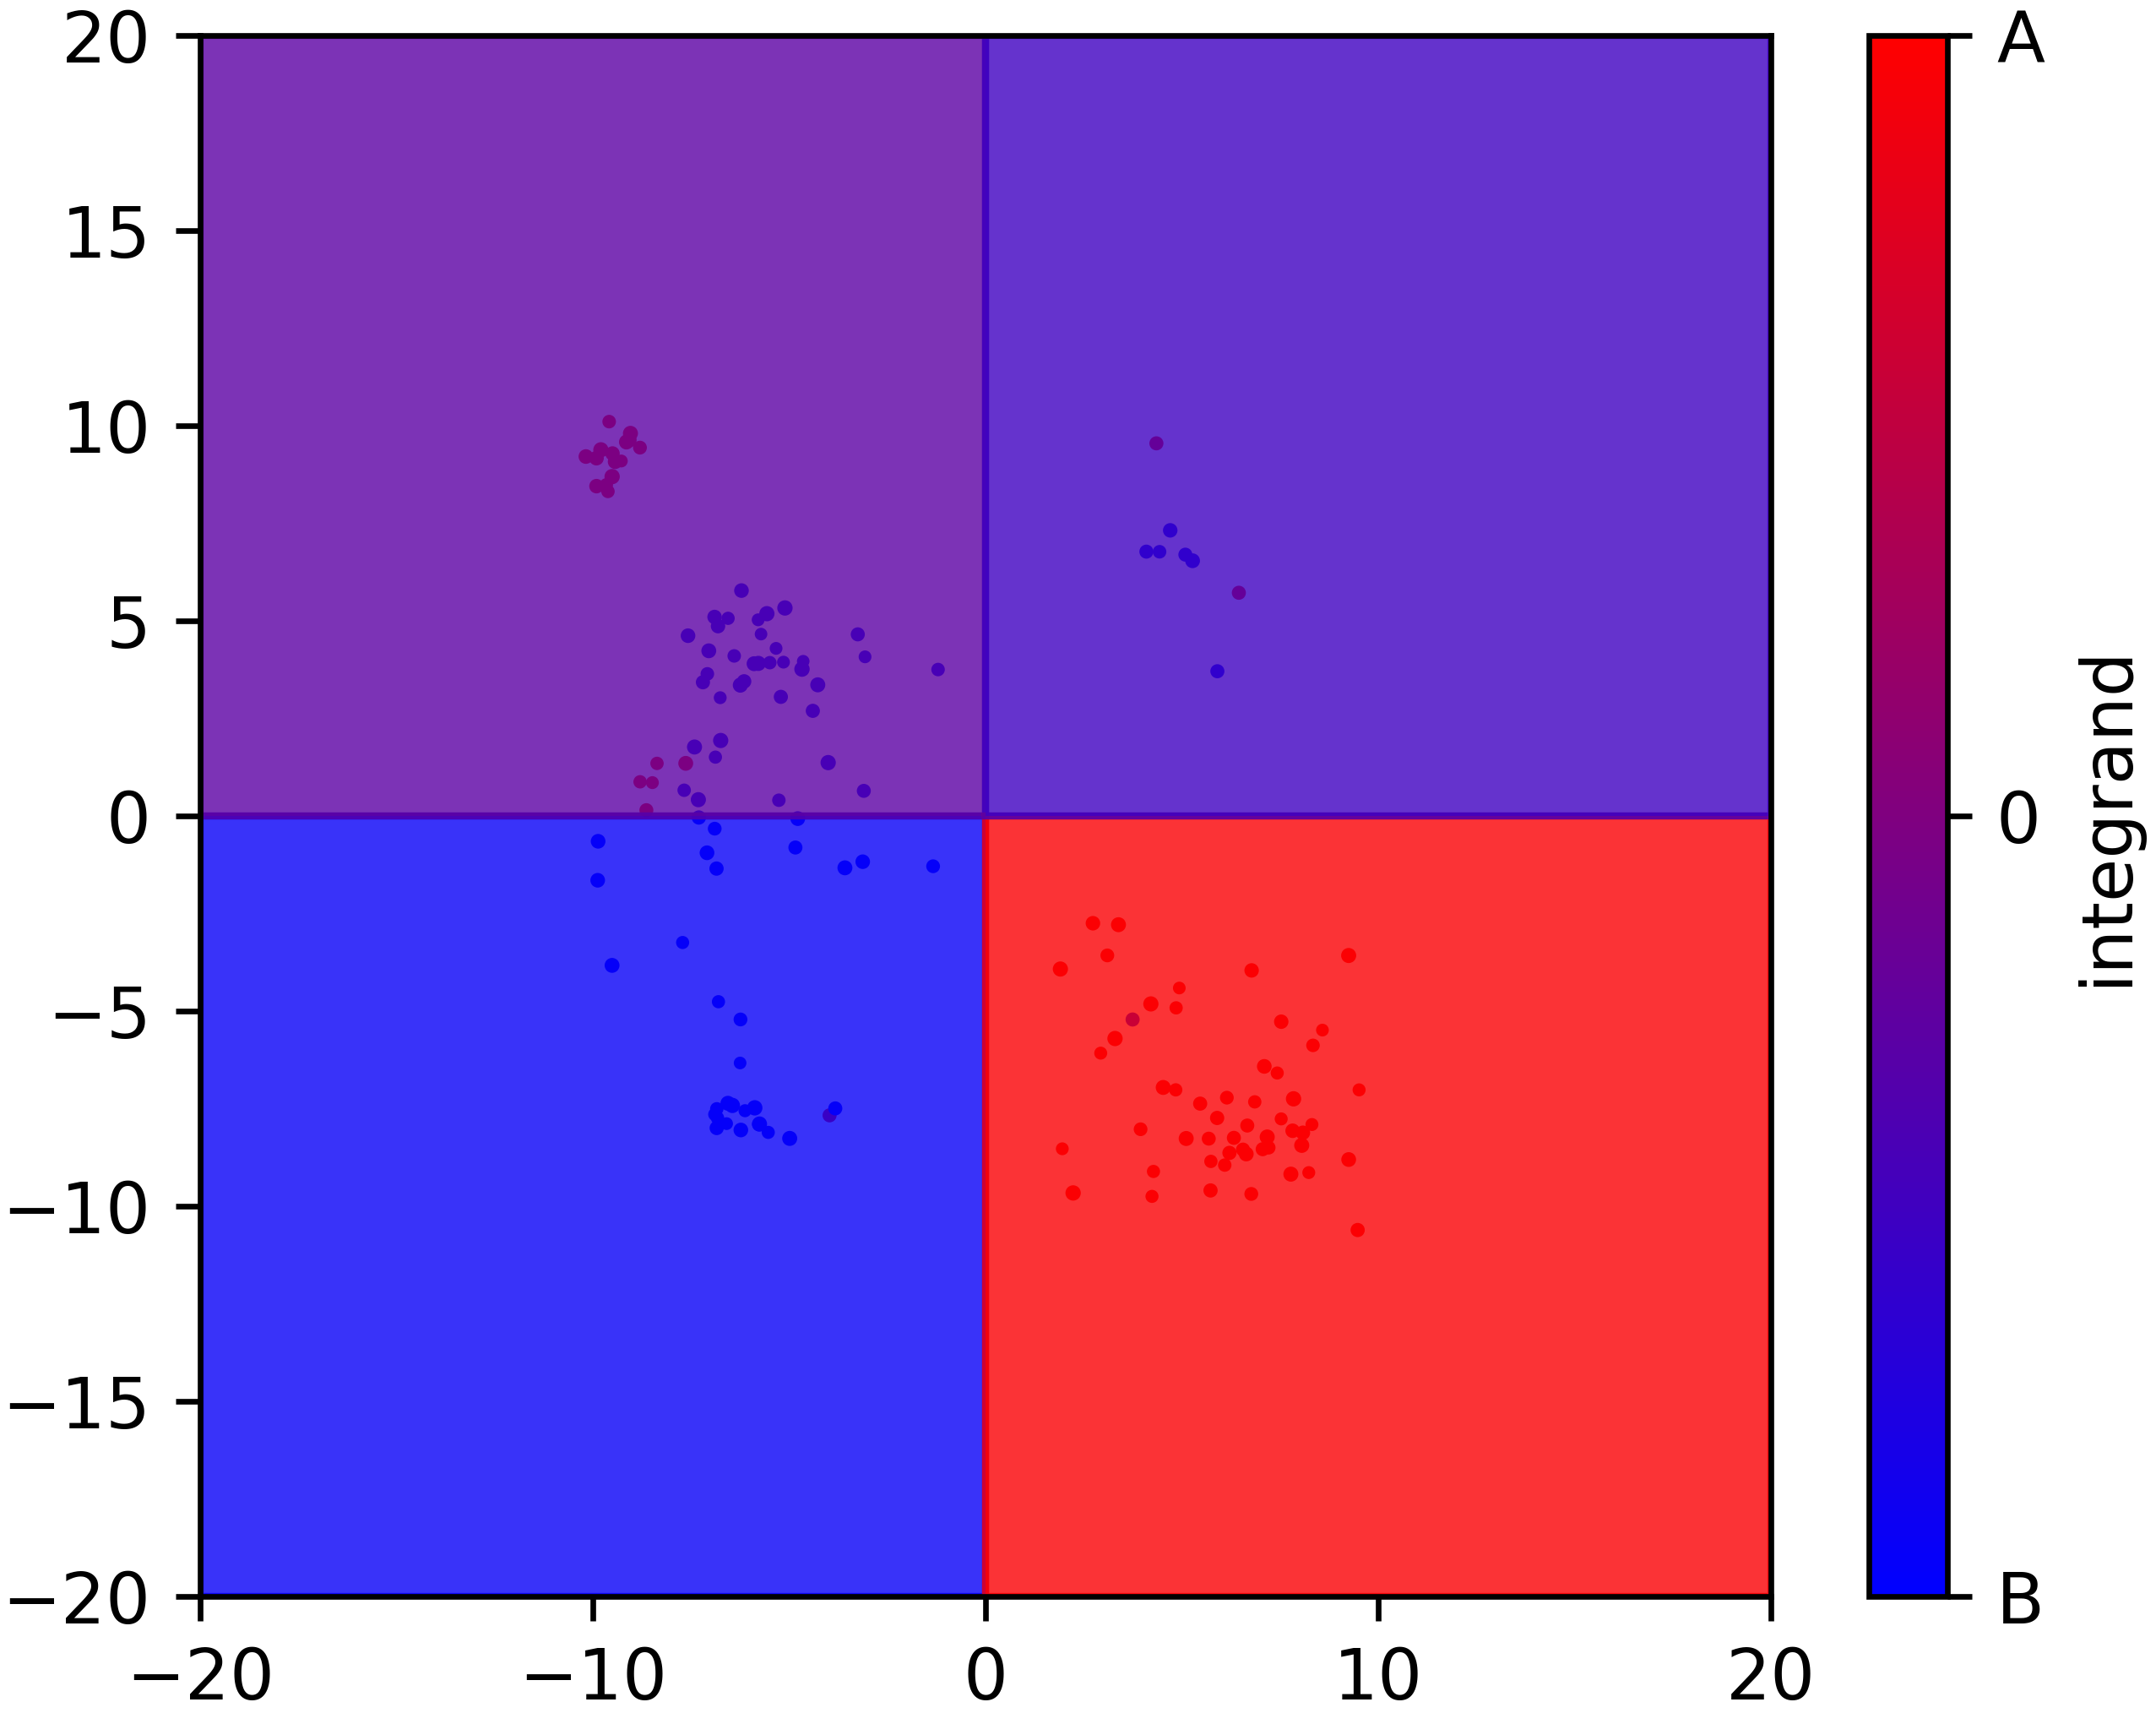
\includegraphics[width=\linewidth]{Figures/box_comparison.png}
		\caption[Box clustering, example of comparison]{Box clustering using $4$ boxes.\\ Computed distance: $0.268$.}
		\label{fig:box_clustering}
	\end{subfigure}
	\hfill
	\begin{subfigure}{0.48\linewidth}
		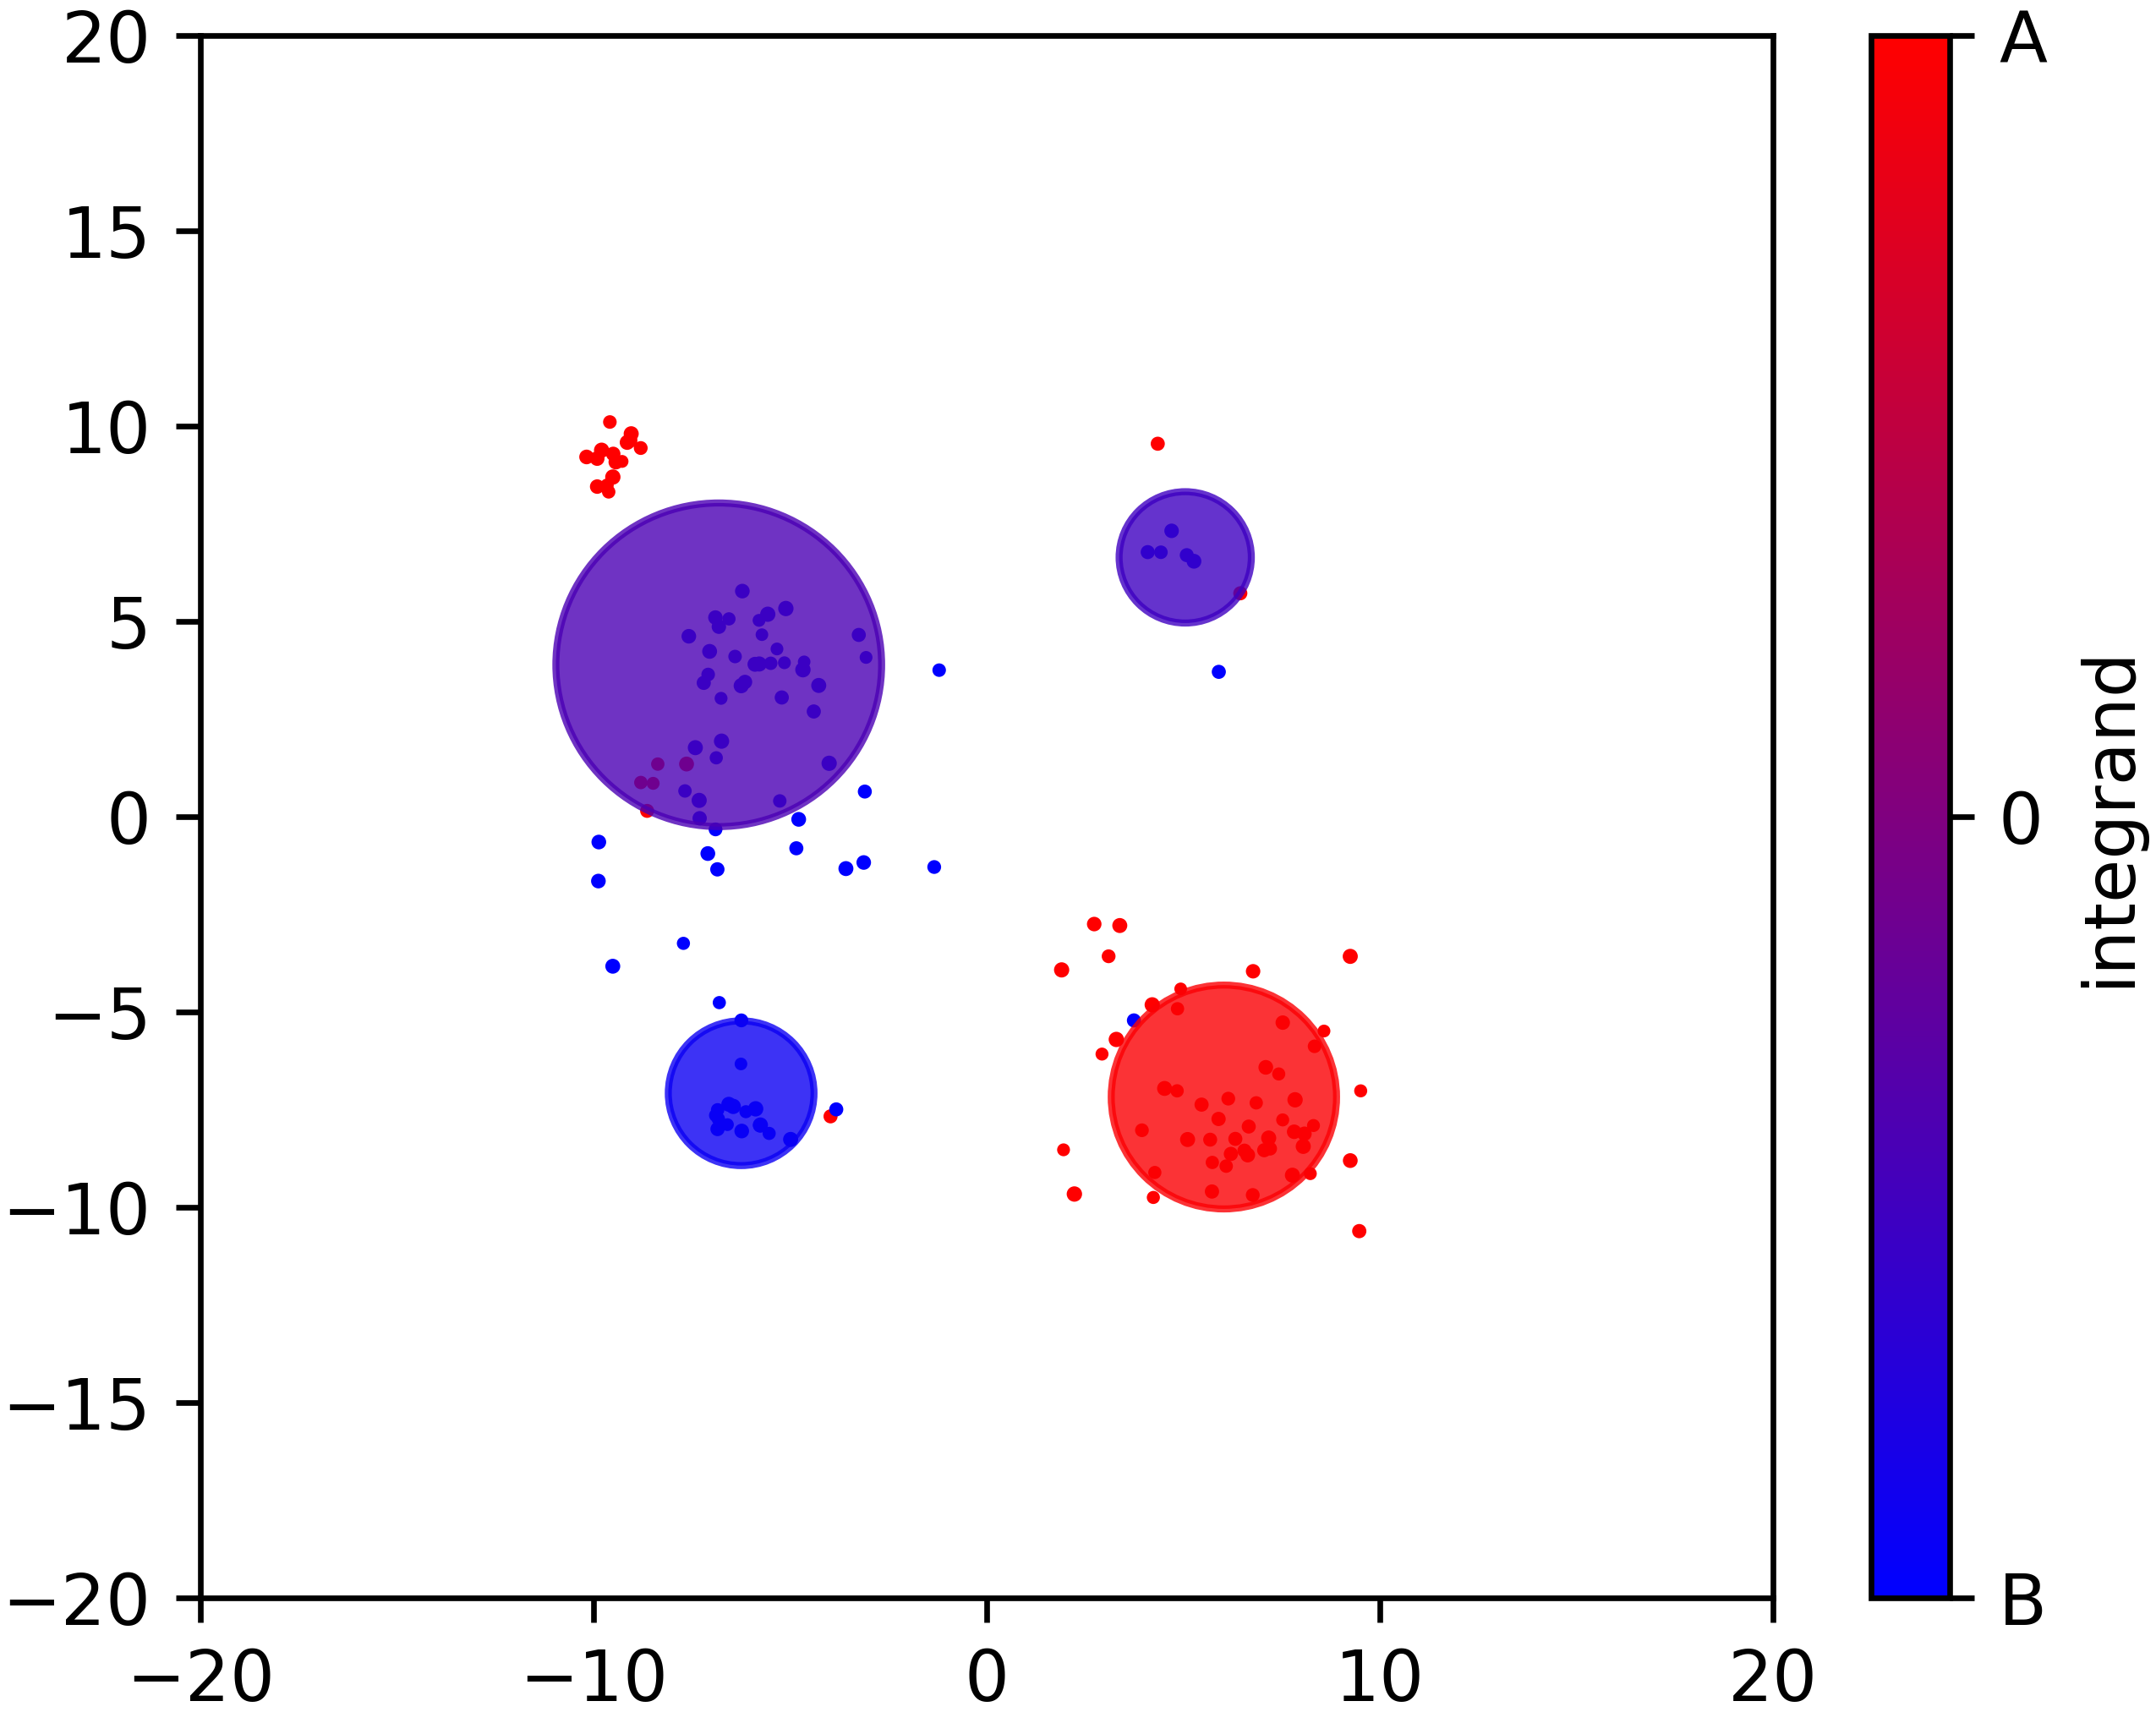
\includegraphics[width=\linewidth]{Figures/kmeans_comparison.png}
		\caption[\gls{kmeans} clustering, example of comparison]{\gls{kmeans} clustering using $4$ centroids.\\ Computed distance: $0.221$.}
		\label{fig:kmeans_clustering}
	\end{subfigure}
	\begin{subfigure}{\linewidth}
		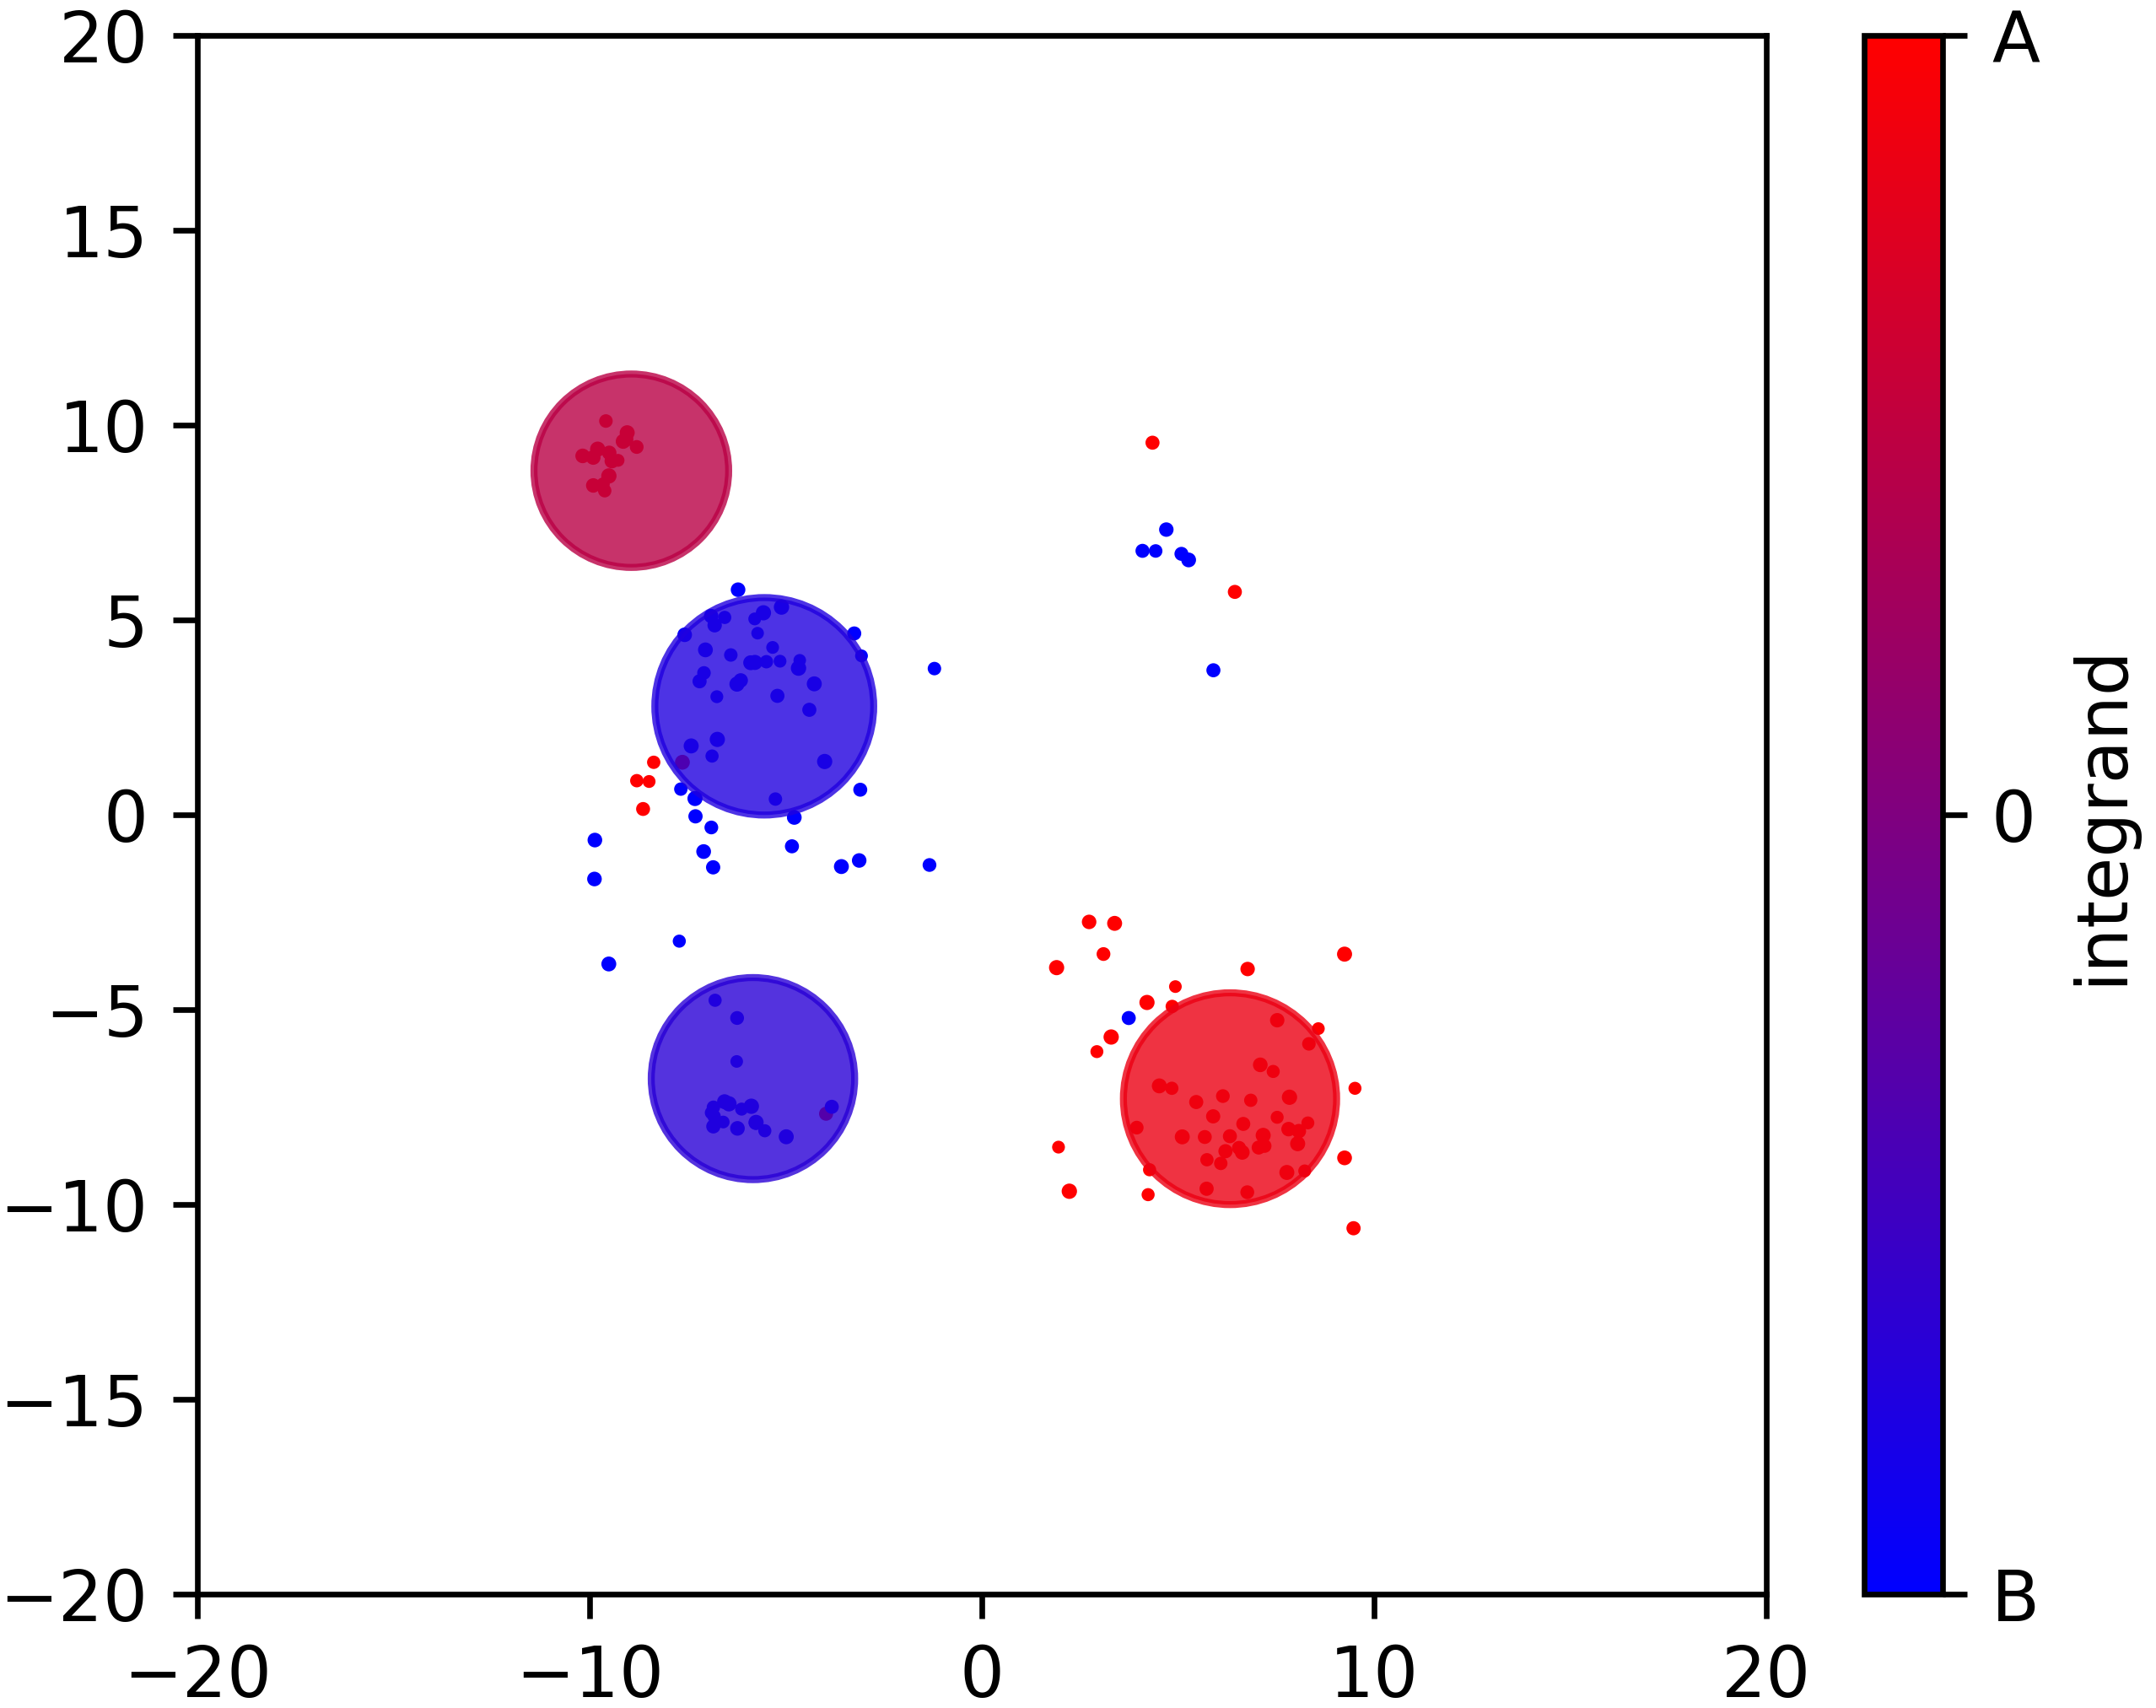
\includegraphics[width=\linewidth]{Figures/fcm_comparison.png}
		\caption[\gls{fcm} clustering, example of comparison]{\gls{fcm} clustering using $4$ centroids.\\ Computed distance $0.289$.}
		\label{fig:fcm_clustering}
	\end{subfigure}
	\caption[example of comparison using $3$ methods]{As can be seen, clusters are assigned a colour that is mapped to $[-1,1]$ ($-1$ is blue, $1$ is red). In particular, this colour is associated with the number $\frac{p_\mathcal{A}(c)-p_\mathcal{B}(c)}{p_\mathcal{A}(c)+p_\mathcal{B}(c)}$ for each cluster of centroid $c$. Furthermore, it is observed that $\gls{kmeans}$ and $\gls{fcm}$ have clusters represented by a circle with area $\mu(c)$ for the two clustering methods.}
\end{figure}
\end{modified}

\begin{modified}
\noindent In order to see the different perspective, we compare the different values obtained from box-clustering, \gls{kmeans} and \gls{fcm}.

\begin{table}[h]
	\centering
	\begin{tabular}{|>{\columncolor{pink}}c|c|c|c|}
		\hline
		\rowcolor{lavender}
		\cellcolor{mint} Values & Box-Clustering & \gls{kmeans} & \gls{fcm} \\
		$\left|D_\mathcal{A}\cap D_\mathcal{B}\right|$ & $4$ & $4$ & $2.889$ \\
		\hline
		$\left|D_\mathcal{A}\cup D_\mathcal{B}\right|$ & $4$ & $4$ & $3.980$ \\
		\hline
		$J_{D_\mathcal{A}, D_\mathcal{B}}$ & $1$ & $1$ & $0.7259$ \\
		\hline
		$\left(1+J_{D_\mathcal{A}, D_\mathcal{B}}\right)^{-1}$ & $0.5$ & $0.5$ & $0.5794$ \\
		\hline
		Integral & $0.5368$ & $0.4418$ & $0.4980$ \\
		\hline
		$d(\mathcal{A},\mathcal{B})$ & $0.268$ & $0.221$ & $0.289$ \\
		\hline
	\end{tabular}
	\caption[Summary of comparison]{Comparing the values obtained from the $3$ algorithms, one can see how \gls{fcm} manages to provide a similar result using fuzzy logic.}
\end{table}
\end{modified}
\begin{toReview}
\begin{exempli_gratia}[Stability of \gls{fcm}]
	Consider a high-dimensional example comparing two sets of samples drawn from two Gaussian distributions with the gradual addition of uniform noise.

	\noindent The goal is to evaluate how noise affects the results obtained from \gls{fcm} compared to \gls{kmeans}.

	\noindent Specifically, we draw two sets of samples from the Gaussian distributions \(\mathcal{N}\left(-\vec{1}, \mathds{1}\right)\) and \(\mathcal{N}\left(\vec{1}, \mathds{1}\right)\) in \(\mathbb{R}^{16}\). Uniform noise with distribution \(\textit{Unif}\left[-5, 5\right]^{16}\) is then added to the data.

	\noindent Each dataset consists of \(500\) samples, combining points from the Gaussian distributions and the noise. The table below shows how the distances between the two distributions decrease as the noise density increases.

	\begin{minipage}{\textwidth}
		\centering
		\begin{tabular}{|>{\columncolor{pink}}c|c|c|}
			\hline
			\rowcolor{lavender}
			\cellcolor{mint} Noise Density & \gls{kmeans} Distance & \gls{fcm} Distance \\
			$0\%$ & $1.000$ & $0.2975$ \\
			\hline
			$1\%$ & $0.5669$ & $0.2427$ \\
			\hline
			$2\%$ & $0.4858$ & $0.2411$ \\
			\hline
			$5\%$ & $0.4076$ & $0.2247$ \\
			\hline
			$10\%$ & $0.0491$ & $0.1921$ \\
			\hline
			$20\%$ & $0.0054$ & $0.1302$ \\
			\hline
		\end{tabular}
	\end{minipage}

	\noindent The results demonstrate that \gls{fcm} is significantly more robust than \gls{kmeans}, as it maintains a discernible distance between the two Gaussian distributions even in the presence of high noise density.
\end{exempli_gratia}
\end{toReview}

\paragraph{\gls{gpu}}
%L'algoritmo presentato è una soluzione sequenziale per l'estrazione delle tessere. Esso lavora iterando attraverso le righe e le colonne dell'immagine, estrae le tessere di dimensioni $N \times N$ e le inserisce in una lista. Tuttavia, questo approccio ha un costo computazionale pari a $O(hwN^2)$.\\
\noindent The \cref{alg:MembershipUpdateSafe} shown is a sequential solution for \gls{fcm}. It works by iterating through the data and centroids to compute the membership matrix. However, this approach has a computational cost of $O(NCk)$.

%Per migliorare l'efficienza computazionale, si può ricorrere all'utilizzo del boost della GPU (General Purpose Graphics Processing Unit). Questo genere di operazioni è noto come GPGPU (General-Purpose computing on Graphics Processing Units). Sfruttare la potenza di calcolo parallelo offerta dalle GPU può notevolmente accelerare il processo di estrazione delle tessere.
\noindent To improve computational efficiency, the use of \gls{gpu} \gls{boost}ing can be employed. This kind of operation is known as \gls{gpgpu}. Exploiting the parallel computing power offered by a \gls{gpu} can greatly accelerate the process of comparison.

%La \gls{gpu}, o unità di elaborazione grafica, è un componente elettronico presente in ogni computer, in grado di eseguire un grande numero di operazioni in parallelo. Originariamente concepita per gestire l'interfaccia grafica nei videogiochi, la \gls{gpu} si trova tipicamente nelle schede grafiche, dove è in grado di visualizzare miliardi di pixel sullo schermo di ogni computer a velocità che la \gls{cpu} non può raggiungere.\\
\noindent The \gls{gpu} is an electronic component present in every computer, able to perform a large number of operations in parallel. Originally designed to handle the graphical interface in video games, the \gls{gpu} is capable of handling billions of pixels on any computer screen at speeds that the \gls{cpu} cannot achieve.

%Questo processore è costituito da migliaia di thread, organizzati gerarchicamente a livello hardware per massimizzarne le prestazioni:
%\begin{enumerate}[label=\roman*.]
%\item \gls{sm}: Esegue un kernel e consiste di numerosi warp;
%\item \gls{warp}: Esegue il kernel del suo stream e possiede una memoria condivisa tra i suoi thread, di solito $32$;
%\item \gls{thread}: Esegue il kernel del suo warp sincronizzandosi con gli altri \gls{thread} dello stesso \gls{warp} e possiede una propria memoria riservata nei suoi registri.
%\end{enumerate}
\noindent This processor is made up of thousands of threads, organised hierarchically at the hardware level to maximise performance:
\begin{enumerate}[label=\roman*.]
\item \gls{sm}: Runs a kernel and consists of numerous \gls{warp}s;
\item \gls{warp}: Runs the kernel of its stream and has shared memory between its threads, usually $32$;
\item \gls{thread}: Executes the kernel of its warp by synchronising with the other \gls{thread}s of the same \gls{warp} and has its own reserved memory in its registers.
\end{enumerate}
%La memoria alla quale può accedere una \gls{gpu} è suddivisa in diverse categorie, tra cui la memoria \textit{global}, \textit{shared}, \textit{cache} e \textit{register}. L'accesso a queste memorie da parte dei \gls{thread} del processore dipende dalla gerarchia dei \gls{thread} stessi. Ad esempio, la memoria \textit{global} è accessibile da ogni \gls{thread}, mentre la memoria \textit{shared} è accessibile solo dai \gls{thread} appartenenti allo stesso \gls{warp}.\\
\noindent The memory that a \gls{gpu} can access is divided into different categories, namely \textit{global}, \textit{shared}, \textit{cache} and \textit{register} memory. Access to these memories by the processor's \gls{thread}s depends on the hierarchy of the \gls{thread}s themselves. For example, the \textit{global} memory is accessible by every \gls{thread}, while the \textit{shared} memory is only accessible by \gls{thread}s in the same \gls{warp}.

%In un computer di alta fascia, è comune trovare schede video dotate di $14$ \gls{sm}, ognuno dei quali contiene $1024$ \gls{thread} suddivisi in $32$ \gls{warp}. Questo totale di $14336$ \gls{thread} può eseguire in parallelo lo stesso identico codice, consentendo un'elaborazione estremamente veloce delle immagini e di altre operazioni che richiedono un alto grado di parallelismo.\\
\noindent In a high-end computer, it is common to find a \gls{gpu} with dozens of \gls{sm}, each containing $64$ or $128$ \gls{core}s. For example, if a process wants to use $\num{1024}$ threads on a single \gls{sm}, the \gls{gpu} will divide these threads into $32$ warps (each containing $32$ threads). Each warp is executed in chunks of $64$ threads at a time, meaning that $2$ warps can be executed simultaneously per clock cycle, while the remaining warps are scheduled for execution in subsequent cycles. This total of tens of thousands of \gls{thread}s can execute the exact same code in parallel, permitting extremely fast processing of images and other operations requiring a high degree of parallelism.

%A partire dagli anni $2000$, l'uso delle \gls{gpu} si è esteso al campo del calcolo scientifico, introducendo importati concetti come la scalabilità e l'\gls{hpc}. Dal $2020$, sono disponibili sul mercato \gls{gpu} dedicate alle operazioni di intelligenza artificiale.\\
\noindent Since the $2000$s, the use of \gls{gpu} has extended to the field of scientific computing, introducing important concepts such as scalability and \gls{hpc}. Since $2020$, dedicated \gls{gpu} are available on the market for artificial intelligence operations.

%In \gls{Python}, esistono framework utili per l'utilizzo delle \gls{gpu}, come \textit{torch} e \textit{TensorFlow}, ampiamente impiegati nell'ambito della computer vision. Tuttavia, anche linguaggi come il \verb"C++" offrono dialetti che consentono di sfruttare queste potenti unità di calcolo. In questo contesto, si userà il dialetto CUDA.\\
\noindent In \gls{Python}, there are useful frameworks for the utilisation of \gls{gpu}, such as \textit{torch} and \textit{TensorFlow}, which are widely employed in the field of computer vision. However, also languages such as \verb "C++" offer dialects that allow these powerful computing units to be exploited. In this paper, the \gls{cuda} dialect will be used.
\footnote{for more details about GPU architecture, see\newline\url{https://researchcomputing.princeton.edu/support/knowledge-base/gpu-computing}}
\footnote{for more details about \gls{cuda} language, see\newline\url{https://docs.nvidia.com/cuda/}}

\bigskip
The integration of \gls{gpgpu} techniques would allow the workload to be distributed over several cores of the \gls{gpu}, thus reducing the time needed for clustering operations. This method is particularly advantageous when handling large amounts of data, as the \gls{gpu} can perform many operations in parallel, speed up computation to be $2000$ times faster than the \gls{cpu} could have done.

\noindent The sum of $N$ numbers can be performed in with computational cost $O(log(N))$. This is because in parallel the \gls{gpu} threads sum one half of the vector over another at the same instant and then repeat until they get a single component that will have only one number. This operation is called \textit{reduction} and we can see it in the \cref{alg:gpu_reduction}. This is just one detail of how the \gls{gpu} can reduce the asymptotic computational cost of an algorithm. Suffice it to say that thanks to reductions and strong parallelism, it is possible to multiply two $N\times K$ and $K\times M$ matrices with cost $O(log(K))$ instead of $O(NMK)$. In clustering many operations can be parallelised and \gls{fcm} in particular requires many sums and linear operations.

\noindent The limitations of \gls{gpu} are not only related to the execution of the same operations on all threads, but also to the nature of these operations. Normally, an instruction takes much longer to be executed by a \gls{gpu} than by a \gls{cpu}. Arithmetic instructions are the most efficient, while the use of conditions tends to be avoided.

\begin{algorithm}
\caption[Parallel algorithm for sum reduction]{Parallel algorithm for sum reduction.\\
	\begin{minipage}[t]{\linewidth}
		\textsc{INPUT}
		\begin{itemize}[noitemsep, topsep=0pt]
			\item[$\textnormal{v}$:] array of values
			\item[$\textnormal{N}$:] number of components
		\end{itemize}
		This algorithm sum all values of an array and write in $\textnormal{v}[0]$ the result. The array is not preserved, in this way the algorithm does not allocate new memory. The computational cost is $O(\log(N))$. In \cref{fig:gpu_reduction} an example over a vector with $7$ components.
	\end{minipage}
}
\begin{algorithmic}[1]
\Procedure{Kernel $\textnormal{i}$, SumReduction}{$\textnormal{v}$,$\textnormal{N}$}
    \State Let $S$ a shared vector with $2^k \geq N$ component
    \State $S[\textnormal{i}] \gets \textnormal{v}[\textnormal{i}]$ if $\textnormal{i}<\textnormal{N}$ else $0$
    \For{$L \gets 2^{k}/2,2^{k}/4,\dots,1$}
        \If{$\textnormal{i} < L$}
            \State $S[\textnormal{i}] \gets S[\textnormal{i}] + S[\textnormal{i}+L]$
        \EndIf
        \State require synchronisation between threads
    \EndFor
\EndProcedure
\label{alg:gpu_reduction}
\end{algorithmic}
\end{algorithm}

\begin{figure}[h]
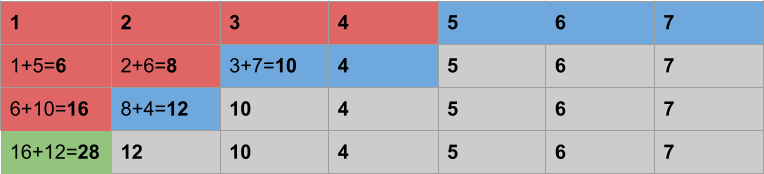
\includegraphics[width=\linewidth]{Figures/example_gpu_reduction.png}
\caption[Application of sum reduction]{We want to calculate the sum of the values in the first row. The idea is to divide the vector into $2$ regions, sum the components, and repeat over the new vector with half the size of the previous vector.}
\label{fig:gpu_reduction}
\end{figure}


% attribution
%\newpage
%\input{main/methodology/Attribution}
